%  LaTeX support: latex@mdpi.com
%  In case you need support, please attach all files that are necessary for compiling as well as the log file, and specify the details of your LaTeX setup (which operating system and LaTeX version / tools you are using).

% You need to save the "mdpi.cls" and "mdpi.bst" files into the same folder as this template file.

%=================================================================
\documentclass[electronics,article,submit,moreauthors,pdftex,10pt,a4paper]{mdpi}
\synctex=1
%\usepackage{fixme}
%\fxsetup{
%    status=draft,
%    author=,
%    %layout=footnote,
%    layout=inline,
%    theme=color
%}
\usepackage{caption}
\usepackage{subcaption}
\usepackage{listings}             % Include the listings-package
\usepackage{placeins}
\usepackage{xcolor}
\usepackage{caption}
\usepackage{textcomp}  % To get the correct quotes in lstlistings (')

\newcommand\floor[1]{\left\lfloor#1\right\rfloor}
\newcommand\ceil[1]{\left\lceil#1\right\rceil}

\newcommand{\todot}[1]{%
  \textcolor{red}{TODO: #1}
}

%--------------------
% Class Options:
%--------------------
% journal
%----------
% Choose between the following MDPI journals:
% actuators, admsci, aerospace, agriculture, agronomy, algorithms, animals, antibiotics, antibodies, antioxidants, applsci, arts, atmosphere, atoms, axioms, batteries, behavsci, beverages, bioengineering, biology, biomedicines, biomimetics, biomolecules, biosensors, brainsci, buildings, carbon, cancers, catalysts, cells, challenges, chemosensors, children, chromatography, climate, coatings, computation, computers, condensedmatter, cosmetics, cryptography, crystals, data, dentistry, designs, diagnostics, diseases, diversity, econometrics, economies, education, electronics, energies, entropy, environments, epigenomes, fermentation, fibers, fishes, fluids, foods, forests, futureinternet, galaxies, games, gels, genealogy, genes, geosciences, geriatrics, healthcare, horticulturae, humanities, hydrology, informatics, information, infrastructures, inorganics, insects, instruments, ijerph, ijfs, ijms, ijgi, inventions, jcdd, jcm, jdb, jfb, jfmk, jimaging, jof, jintelligence, jlpea, jmse, jpm, jrfm, jsan, land, languages, laws, life, literature, lubricants, machines, magnetochemistry, marinedrugs, materials, mathematics, mca, mti, medsci, medicines, membranes, metabolites, metals, microarrays, micromachines, microorganisms, minerals, molbank, molecules, mps, nanomaterials, ncrna, neonatalscreening, nutrients, particles, pathogens, pharmaceuticals, pharmaceutics, pharmacy, philosophies, photonics, plants, polymers, processes, proteomes, publications, recycling, religions, remotesensing, resources, risks, robotics, safety, sensors, separations, sexes, sinusitis, socsci, societies, soils, sports, standards, sustainability, symmetry, systems, technologies, toxics, toxins, universe, urbansci, vaccines, vetsci, viruses, water
%---------
% article
%---------
% The default type of manuscript is article, but can be replaced by:
% addendum, article, book, bookreview, briefreport, casereport, changes, comment, commentary, communication, conceptpaper, correction, conferencereport, expressionofconcern, meetingreport, creative, datadescriptor, discussion, editorial, essay, erratum, hypothesis, interestingimage, letter, newbookreceived, opinion, obituary, projectreport, reply, retraction, review, sciprints, shortnote, supfile, technicalnote
% supfile = supplementary materials
%----------
% submit
%----------
% The class option "submit" will be changed to "accept" by the Editorial Office when the paper is accepted. This will only make changes to the frontpage (e.g. the logo of the journal will get visible), the headings, and the copyright information. Also, line numbering will be removed. Journal info and pagination for accepted papers will also be assigned by the Editorial Office.
%------------------
% moreauthors
%------------------
% If there is only one author the class option oneauthor should be used. Otherwise use the class option moreauthors.
%---------
% pdftex
%---------
% The option pdftex is for use with pdfLaTeX. If eps figure are used, remove the option pdftex and use LaTeX and dvi2pdf.

% *** ACRONYM PACKAGE ***
\usepackage[nolist]{acronym}
% \acf{GS} writes Ground Station
% \ac{GS} writes GS exept for the first time
%syntax: \acro{<acronym>}[<short name>]{<full name>}
\begin{acronym}[]
\acro{3GPP}{3rd Generation Partnership Project}
\acro{6LoWPAN}{IPv6 over Low power Wireless Personal Area Networks}
\acro{ACK}{Acknowledgment}
\acro{AMR}{Adaptive Multi-Rate}
\acro{AP}{Access Point}
\acro{ARM}{Advanced RISC Machine}
\acro{ARQ}{Automatic Repeat-reQuest}
\acro{ARF}{Auto Rate Fallback}
\acro{API}{Application Programming Interface}
\acro{BER}{Bit Error Rate}
\acro{BLAS}{Basic Linear Algebra Subprograms}
\acro{BS}{Base Station}
\acro{BSS}{Basic Service Set}
\acro{cdf}{Cummulative Density Function}
\acro{CFP}{Contention Freeze Periode}
\acro{CPU}{Central Processing Unit}
\acro{CSMA/CA}{Carrier Sense Multiple Access with Collision Avoidance}
\acro{CW}{Contention Window}
\acro{CWN}{Cooperative Wireless Network}
\acro{CTS}{Clear to Send}
\acro{D2D}{Device to Device}
\acro{DAG}{Direct Acyclic Graph}
\acro{DC}{Direct Current}
\acro{DCF}{Distributed Coordination Function}
\acro{DIFS}{Distributed Interframe Space}
\acro{ERP}{Extended Rate PHY}
\acro{FEC}{Forward Error Correction}
\acro{FCS}{Frame Check Sequence}
\acro{FF}{Finite Field}
\acro{GF}{Galois Field}
\acro{GPS}{Global Positioning System}
\acro{GPU}{Graphic Processing Unit}
\acro{HTTP}{Hyper Text Transfer Protocol}
\acro{IBSS}{Independent BSS}
\acro{IC}{Interference Cancellation}
\acro{ICST}{Institute for Computer Sciences, Social-Informatics and Telecommunications Engineering}
\acro{IFS}{Interframe Space}
\acro{IoT}{Internet of Things}
\acro{IP}{Internet Protocol}
\acro{IPTV}{Internet Protocol TeleVision}
\acro{JCN}{Journal of Communications and Networks}
\acro{KL}{Kullback-Leibler}
\acro{LAN}{Local Area Network}
\acro{LDPC}{Low Density Parity Check}
\acro{l.d.}{linearly dependent}
\acro{l.i.}{linearly independent}
\acro{LNC}{Linear Network Coding}
\acro{LOS}{Line Of Sight}
\acro{LTE-A}{Long Term Evolution Advanced}
\acro{MAC}{Medium Access Control}
\acro{MANET}{Mobile Ad hoc NETwork}
\acro{MIMO}{Multiple Input Multiple Output}
\acro{MIT}{Massachusetts Institute of Technology}
\acro{MTBF}{Mean Time Between Failure}
\acro{M2M}{Machine-to-Machine}
\acro{NAV}{Network Allocation Vector}
\acro{NEP}{Nokia Energy Profiler}
\acro{NC}{Network Coding}
\acro{NLOS}{Non Line Of Sight}
\acro{NIC}{Network Interface Card}
\acro{OSI}{Open Systems Interconnect}
\acro{PC}{Personal Computer}
\acro{PDA}{Personal Digital Assistant}
\acro{PEP}{Packet Error Probability}
\acro{pgf}{Probability Generating Function}
\acro{PHY}{Physical Layer}
\acro{PLCP}{Physical Layer Convergence Procedure}
\acro{pmf}{Probability Mass Function}
\acro{PNC}{Physical layer Network Coding}
\acro{PPDU}{PLCP Protocol Data Unit}
\acro{QoE}{Quality of Experience}
\acro{QoS}{Quality of Service}
\acro{RLNC}{Random Linear Network Coding}
\acro{ROC}{Region of Convergence}
\acro{SRLNC}{Sparse Random Linear Network Coding}
\acro{SIMD}{Single Instruction Multiple Data}
\acro{SAIC}{Single Antenna Interference Cancellation}
\acro{SIFS}{Short Interframe Space}
\acro{SIMD}{Single Instruction Multiple Data}
\acro{SINR}{Signal-to-Interference-plus-Noise Ratio}
\acro{SMP}{Symmetric Multiprocessor}
\acro{SNMP}{Simple Network Management Protocol}
\acro{SNR}{Signal-to-Noise Ratio}
\acro{SOC}{System on Chip}
\acro{SSE}{Streaming SIMD Extensions}
\acro{SSID}{Service Set Identifier}
\acro{TSNC}{Tunable Sparse Network Coding}
\acro{UDP}{User Datagram Protocol}
\acro{UML}{Unified Modeling Language}
\acro{UI}{User Interface}
\acro{VANET}{Vehicular Ad-hoc Network}
\acro{VoIP}{Voice over Internet Protocol}
\acro{WBN}{Wireless Broadcast Network}
\acro{WiFi}{Wireless Fidelity}
\acro{WLAN}{Wireless Local Area Network}
\acro{WMN}{Wireless Mesh Network}
\acro{pmf}{Probability Mass Function}
\acro{TC}{Telescopic Codes}
\acro{TBTT}{Target Beacon Transmision Times}
\acro{TCP}{Transmission Control Protocol}
\acro{dof}{degrees of freedom}
\acro{IP}{Internet Protocol}
\acro{OS}{Operating System}
\acro{NFS}{Network File System}
\acro{RAM}{Random Access Memory}
\acro{Raspi}{Raspberry Pi}
\acro{SSH}{Secure Shell}
\acro{USB}{Universal Serial Bus}
\acro{SCP}{Secure copy}
\acro{Telnet}{Telnet}
\acro{GB}{Gigabyte}
\end{acronym}
 % Name of acronyms file

% *** ALGORITHM PACKAGE ***
\usepackage[]{algorithm2e}

% *** PDF PACKAGE *** ..to extract a page from a PDF with multiple pages.
\usepackage{pdfpages}

%=================================================================
\firstpage{1}
\makeatletter
\setcounter{page}{\@firstpage}
\makeatother
\articlenumber{x}
\doinum{10.3390/------}
\pubvolume{xx}
\pubyear{2016}
\copyrightyear{2016}
\externaleditor{Academic Editor: Steven Johnston and Simon J. Cox}
\history{Received: date; Accepted: date; Published: date}
%------------------------------------------------------------------
% The following line should be uncommented if the LaTeX file is uploaded to arXiv.org
%\pdfoutput=1

%=================================================================
% Add packages and commands here. The following packages are loaded in our class file: fontenc, calc, indentfirst, fancyhdr, graphicx, lastpage, ifthen, lineno, float, amsmath, setspace, enumitem, mathpazo, booktabs, titlesec, etoolbox, amsthm, hyphenat, natbib, hyperref, footmisc, geometry, caption, url, mdframed

%=================================================================
%% Please use the following mathematics environments:
 \theoremstyle{mdpi}
 \newcounter{thm}
 \setcounter{thm}{0}
 \newcounter{ex}
 \setcounter{ex}{0}
 \newcounter{re}
 \setcounter{re}{0}

 \newtheorem{Theorem}[thm]{Theorem}
 \newtheorem{Lemma}[thm]{Lemma}
 \newtheorem{Corollary}[thm]{Corollary}
 \newtheorem{Proposition}[thm]{Proposition}

 \theoremstyle{mdpidefinition}
 \newtheorem{Characterization}[thm]{Characterization}
 \newtheorem{Property}[thm]{Property}
 \newtheorem{Problem}[thm]{Problem}
 \newtheorem{Example}[ex]{Example}
 \newtheorem{ExamplesandDefinitions}[ex]{Examples and Definitions}
 \newtheorem{Remark}[re]{Remark}
 \newtheorem{Definition}[thm]{Definition}
%% For proofs, please use the proof environment (the amsthm package is loaded by the MDPI class).

%=================================================================
% Full title of the paper (Capitalized)
\Title{On Goodput and Energy Measurements of \\ Network Coding Schemes in the Raspberry Pi}

% Authors, for the paper (add full first names)
\Author{N\'estor J. Hern\'andez Marcano $^{1,2,\dagger}$*, Chres W. S{\o}rensen $^{2,\dagger}$, Juan A. Cabrera G. $^{3,4}$, Simon Wunderlich $^{3}$, Daniel E. Lucani $^{2,\dagger}$ and Frank H. P. Fitzek $^{3}$}
% Authors, for metadata in PDF
\AuthorNames{Chres W. Soerensen, Nestor J. Hernandez M., Juan Cabrera, Simon Wunderlich, Daniel E. Lucani and Frank H. P. Fitzek}
% Affiliations / Addresses (Add [1] after \address if there is only one affiliation.)
\address{%
$^{1}$ \quad Steinwurf ApS. Aalborg, Denmark; nestor@steinwurf.com\\
$^{2}$ \quad Aalborg University, Department of Electronic Systems. Aalborg, Denmark; \{nh, cws, del\}@es.aau.dk\\
$^{3}$ \quad Technische Universit\"at Dresden, Deutsche Telekom Chair of Communication Networks. Dresden, Germany; \{juan.cabrera, frank.fitzek\}@tu-dresden.de, simon.wunderlich@mailbox.tu-dresden.de\\
$^{4}$ \quad SFB 912 -- Collaborative Research Center HAEC. Dresden, Germany}

% Contact information of the corresponding author
\corres{Correspondence: nestor@steinwurf.com, nh@es.aau.dk; Tel.: +45 51 20 03 49}

% Current address and/or shared authorship
\firstnote{Fredrik Bajers Vej 7A, Room A3-110. Aalborg, Denmark}

% Simple summary
%\simplesumm{}

% Abstract (Do not use inserted blank lines, i.e. \\)
\abstract{Given that next generation networks are expected to be populated
by a large number of devices, there is a need for quick deployment and
evaluation of alternative mechanisms to cope with the possible generated
traffic in large-scale distributed data networks. In this sense, the
Raspberry Pi has been a popular network node choice due to its reduced
size, processing capabilities, low cost and its support by
widely-used operating systems. For information transport, network coding is
a new paradigm for fast and reliable data processing in networking and
storage systems which overcomes various limitations of state-of-the-art
routing techniques. Therefore, in this work we provide an in-depth
performance evaluation of \ac{RLNC} based schemes for the Raspberry Pi
models 1 and 2, by showing the processing speed of the encoding and
decoding operations and the corresponding energy consumption. Our
results show that, in several scenarios, processing speeds of more
than 80 Mbps in the Raspberry Pi model 1 and 800 Mbps in the Raspberry
Pi model 2 are attainable. Moreover, we show that the processing
energy per bit for network coding is below 1 nJ or even an order of
magnitude less in these scenarios.}

% A single paragraph of about 200 words maximum. For research articles, abstracts should give a pertinent overview of the work. We strongly encourage authors to use the following style of structured abstracts, but without headings: 1) Background: Place the question addressed in a broad context and highlight the purpose of the study; 2) Methods: Describe briefly the main methods or treatments applied; 3) Results: Summarize the article's main findings; and 4) Conclusion: Indicate the main conclusions or interpretations. The abstract should be an objective representation of the article: it must not contain results which are not presented and substantiated in the main text and should not exaggerate the main conclusions.

% Keywords
\keyword{Network Coding; Raspberry Pi; Goodput; Energy; Performance}

% keyword 1; keyword 2; keyword 3. List three to ten pertinent keywords specific to the article, yet reasonably common within the subject discipline.

% The fields PACS, MSC, and JEL may be left empty or commented out if not applicable
%\PACS{J0101}
%\MSC{}
%\JEL{}

% If this is an expanded version of a conference paper, please cite it here: enter the full citation of your conference paper, and add $^\S$ in the end of the title of this article.
%\conference{}

%%%%%%%%%%%%%%%%%%%%%%%%%%%%%%%%%%%%%%%%%%
% Only for the journal Data:

%\dataset{DOI number or link to the deposited data set in cases where the data set is published or set to be published separately. If the data set is submitted and will be published as a supplement to this paper in the journal Data, this field will be filled by the editors of the journal. In this case, please make sure to submit the data set as a supplement when entering your manuscript into our manuscript editorial system.}

%\datasetlicense{license under which the data set is made available (CC0, CC-BY, CC-BY-SA, CC-BY-NC, etc.)}

%%%%%%%%%%%%%%%%%%%%%%%%%%%%%%%%%%%%%%%%%%
\begin{document}
\definecolor{mygreen}{rgb}{0,0.6,0}
\definecolor{mygray}{rgb}{0.5,0.5,0.5}
\definecolor{mymauve}{rgb}{0.58,0,0.82}
\lstset{ %
  backgroundcolor=\color{white},   % choose the background color; you must add \usepackage{color} or \usepackage{xcolor}
  basicstyle=\footnotesize\ttfamily,
  breakatwhitespace=false,         % sets if automatic breaks should only happen at whitespace
  breaklines=true,                 % sets automatic line breaking
  captionpos=b,                    % sets the caption-position to bottom
  %commentstyle=\color{mygreen},    % comment style
  deletekeywords={...},            % if you want to delete keywords from the given language
  %escapeinside={\%*}{*)},          % if you want to add LaTeX within your code
  escapeinside={<@}{@>},
  extendedchars=true,              % lets you use non-ASCII characters; for 8-bits encodings only, does not work with UTF-8
  frame=single,	                   % adds a frame around the code
  keepspaces=true,                 % keeps spaces in text, useful for keeping indentation of code (possibly needs columns=flexible)
  %keywordstyle=\color{blue},       % keyword style
  %language=Bash,                 % the language of the code
  otherkeywords={*,...},           % if you want to add more keywords to the set
  numbers=left,                    % where to put the line-numbers; possible values are (none, left, right)
  numbersep=5pt,                   % how far the line-numbers are from the code
  numberstyle=\tiny\color{mygray}, % the style that is used for the line-numbers
  rulecolor=\color{black},         % if not set, the frame-color may be changed on line-breaks within not-black text (e.g. comments (green here))
  showspaces=false,                % show spaces everywhere adding particular underscores; it overrides 'showstringspaces'
  showstringspaces=false,          % underline spaces within strings only
  showtabs=false,                  % show tabs within strings adding particular underscores
  stepnumber=1,                    % the step between two line-numbers. If it's 1, each line will be numbered
  %stringstyle=\color{mymauve},     % string literal style
  tabsize=2,	                   % sets default tabsize to 2 spaces
  title=\lstname,                  % show the filename of files included with \lstinputlisting; also try caption instead of title
  xleftmargin=5mm,
  xrightmargin=5mm,
  columns=flexible,
  upquote=true
}

% Used to suppress line numbers in lstlistings
\let\origthelstnumber\thelstnumber
\makeatletter
\newcommand*\Suppressnumber{%
  \lst@AddToHook{OnNewLine}{%
    \let\thelstnumber\relax%
     \advance\c@lstnumber-\@ne\relax%
    }%
}

% Used to reactivate line numbers in lstlistrings
\newcommand*\Reactivatenumber{%
  \lst@AddToHook{OnNewLine}{%
   \let\thelstnumber\origthelstnumber%
   \advance\c@lstnumber\@ne\relax}%
}


%%%%%%%%%%%%%%%%%%%%%%%%%%%%%%%%%%%%%%%%%%
%% Sections that are not mandatory are listed as such. The section titles given are for Articles. Review papers and other article types have a more flexible structure.

%% Only for the journal Gels: Please place the Experimental Section after the Conclusions

%%%%%%%%%%%%%%%%%%%%%%%%%%%%%%%%%%%%%%%%%%
% \setcounter{section}{-1} %% Remove this when starting to work on the template.
% \section{How to Use this Template}

% The template details the sections that can be used in a manuscript. Sections that are not mandatory are listed as such. The section titles given are for Articles. Review papers and other article types have a more flexible structure. For any questions, please contact the editorial office of the journal or support@mdpi.com. For LaTeX related questions please contact Janine Daum at latex-support@mdpi.com.

\section{Introduction}
%!TEX root = raspi_journal.tex
% At the beginning, there was darkness and then... bang! \ac{NC}
% \cite{ahlswede2000network} appeared to save us from the evilness
% of routing.
%
% General introduction. Introduction to topic addressed in the journal.
% Review of the State of the Art. Specify why our approach has benefits
% and which are they. Indicate contributions.

% RAW INTRODUCTION: NEED OF DISTRIBUTED NETWORKS AND THE RASPBERRY PI
Due to the advent of the \ac{IoT}, approximately 50 billion devices
ranging from sensors to phones are expected to be connected through
data networks in relatively short period of time \cite{cisco2011forecast}.
This massive deployment requires the design and testing of new
distributed systems that permit to manage the amount of traffic
from the proposed services provided by these devices. Therefore,
development platforms that help to quickly deploy, analyze and
evaluate this type of settings are highly desirable for research.
The emergence of a powerful and inexpensive portable computer such
as the Raspberry Pi, running standard operating systems such as
Linux or Windows, allows to achieve this goal since it enables the
deployment of distributed systems in a rapid fashion at a low cost.
Also, the use of an operating system that has a large user community
permits to administrative these networks in a flexible, stable and
supported fashion.

% INTRODUCTION TO NETWORK CODING
Introduced in~\cite{ahlswede2000network}, \ac{NC}
constitutes a paradigm shift in the way networks are understood
by changing how information is sent through them.
Instead of treating the packets as atomic
unmodifiable units, packets are seen as algebraic entities in a \ac{GF}
that can be operated on to create new coded packets. This permits to
remove the limitation of sending \textit{specific} packets by now sending
coded packets as \textit{linear equations} of the original ones. This
change in the way of seeing how the data is represented, brings new
features that can be exploited. In this way, instead of typically encoding
and decoding on a hop basis, relaying nodes can take part in the
coding process without needing to decode. Therefore, a relay can
\textit{recode} packets, i.e. encode again previously received encoded
(but not decoded) packets in order to reduce delay and still
take advantage of the data representation for the next hop.

Compared to other broadly used coding schemes, e.g. \ac{LDPC}
codes~\cite{gallager1962low} or Reed-Solomon
codes~\cite{reed1960polynomial}, network coding is a technology that
has been implemented in real systems since the early years of its
conception. Authors in~\cite{katti2008xors} showed the
performance of the COPE protocol for the two-way relay channel
in a wireless network, which relied on minimalistic coding and obtaining
gains over a forwarding scheme. Later, the work in~\cite{pedersen2008implementation} used commercially available
Symbian OS mobile phones to implement network coding in a
\ac{D2D} cooperation-based application. Furthermore,
in~\cite{kodo2011pedersen}, the Kodo library was introduce. Kodo is
a C++11 network coding library intended to make network coding
basic functionalities easily available for both the research community
and commercial entities. Based on Kodo, the CATWOMAN
protocol~\cite{hundeboll2012catwoman} is implemented on top of the
BATMAN protocol~\cite{johnson2008simple} for WiFi multi-hop meshed
networks. It uses some of the intuition from COPE, but it is deployed
within the X topology with overhearing links. Its source code is available
as open source in the Linux kernel. Moreover, many other successful
implementations have been tested on real world systems such as
found in~\cite{pahlevani2013playncool,krigslund2013core,
paramanathan2013leanandmean}. For the Raspberry Pi platform, an evaluation
of the performance of \ac{RLNC} can be found in \cite{paramanathan2014sharing}.
However, this evaluation focused particularly on observing the achievable
speeds with \ac{RLNC} \cite{ho2006random} by different configurations of
the code parameters with a single thread and no hardware acceleration through
\ac{SIMD}.

In this work, we provide detailed measurements of the goodput (processing
speed) and energy consumption of \ac{Raspi} models 1 and 2, when
performing network coding operations with different codecs based on \ac{RLNC}
such as: full dense \ac{RLNC}, multicore-enabled \ac{RLNC}, sparse \ac{RLNC}
and tunable sparse \ac{RLNC}. For these coding schemes, the encoder and implementations from Kodo now detect and exploit the \ac{SIMD}
capabilities of the Raspberry Pi. We also assess the \ac{Raspi}
performance excluding the effect of packet losses or delays in order to have a
description of the codes in terms of their parameters. To achieve this,
we perform a measurement campaign with the indicated coding schemes and
their parameters in our local Raspberry Pi testbed. Our measurements permit
us to characterize the goodput and energy consumption
of these devices showing that speeds of 800 Mbps and processing energy per bit
values of 0.1 nJ are possible. Our work is organized as follows.
Section~\ref{sec:schemes} defines the
coding schemes employed in our study. Later, in Section~\ref{sec:metrics}
we describe the considered metrics and methodology for performance comparison
of the codes deployed in the \ac{Raspi}. In Section~\ref{sec:measurements}, we
show the measurements in the \ac{Raspi} models of the mentioned metrics
providing full discussions about the observed operational regimes and effects.
Final conclusions and future work are reviewed in
Section~\ref{sec:conclusions}.

%The introduction should briefly place the study in a broad context and highlight why it is important. It should define the purpose of the work and its significance. The current state of the research field should be reviewed carefully and key publications should be cited. Please highlight controversial and diverging hypotheses when necessary. Finally, briefly mention the main aim of the work and highlight the main conclusions. As far as possible, please keep the introduction comprehensible to scientists outside your particular field of research.


% \section{Testbed Description}
% \input{testbed}

% \section{Cross-compilation: From PC to Raspberry Pi}
% \input{cross_compilation}

\section{Coding Schemes}
%!TEX root = raspi_journal.tex
\label{sec:schemes}

In this section, we present the considered coding schemes that are evaluated
in the \ac{Raspi} 1 and 2.
%In this section, we present a description of the considered coding
%schemes measured with the \ac{Raspi} testbed.
We introduce a
definition for the primitive coding operations, e.g. encoding,
decoding and recoding (where it applies) for each coding
scheme. Later, we address particular schemes which are obtained by
modifying the basic coding operations that provide better processing
speeds, which is particularly relevant for the \ac{Raspi}.  Finally,
we include a review of algorithms for network coding that exploit
multicore capabilities of the \ac{Raspi} 2.


\subsection{Random Linear Network Coding}
\label{ssec:RLNC}

\ac{RLNC} is an example of intra-session \ac{NC}, i.e., data symbols
from a single flow are combined with each other. In this type of
network coding, all the original data packets $P_j, j \in [1,g]$, each
of $B$ bytes, are used to create coded packets using random linear
combinations of the original ones. In the following subsections, we
describe the basic functionalities of \ac{RLNC}.

\subsubsection{Encoding}
In \ac{RLNC}, any coded packet is a linear combination of all
the original packets. For the coding scheme, packets are seen as
algebraic entities formed as a sequence of elements from $GF(q)$,
which is a \ac{GF} of size $q$. Later, each original packet is
multiplied by a coding coefficient from $GF(q)$. The coding coefficients
are chosen uniformly at random from the \ac{GF} by the encoder. To
perform the multiplication of a packet by a coding coefficient, the
coefficient is multiplied for each of the elements in the
concatenation that composes an original packet, preserving the
concatenation. Later, all resulting packets are added within the
\ac{GF} arithmetics together to generate a coded packet. Thus, a
coded packet can be written as:
%
\begin{align} \label{eq:coded_packet}
C_i  &= \bigoplus_{j=1}^{g} v_{ij} \otimes P_j ,\ \forall i \in [1,\ldots)
\end{align}

In \eqref{eq:coded_packet}, $C_i$ is the generic coded packet. In principle,
the encoder may produce any number of coded packets, but a finite
number is produced in practice given that a decoder needs only
$g$ \ac{l.i.} coded packets to decode the batch. Also, in
\eqref{eq:coded_packet}, $v_{ij}$ is the coding coefficient used in the
$i$-th coded packet and assigned to multiply the $j$-th original packet.

For indicating to a receiver how the packets were combined
to create a coded one, a simple yet versatile choice is to append
its coding coefficients as a header in the coded packet. Hence, an
amount of overhead is included in every coded packet given that we
need to provide some signaling needed for decoding. The coding
coefficients overhead amount for packet $i$, $|v_i|$, can be quantified
as:
%
\begin{align} \label{eq:coded_packet_coef}
|v_i| &= \sum_{j=1}^{g} |v_{ij}| = g \times \lceil \log_{2} (q)
\rceil ~ [\mathrm{bits}].
\end{align}

\subsubsection{Decoding}
\label{sssec:decoding}
To be able to decode a batch of $g$ packets, a \ac{l.i.} set of $g$
coded packets, $C_i,\ i \in [1,g]$ is required at a decoder.
Once this set has been collected for a decoder,
the original packets can be found by computing the solution of a system
of linear equations using \ac{GF} aritmethics. Thus, we define
$\textbf{C} = \left[C_1 \ldots C_g \right]^T$,
$\textbf{P} = \left[P_1 \ldots P_g \right]^T$ and the coding matrix
$\textbf{V}$ that collects the coding coefficients for each of the $g$
coded packets, as follows:
%
\begin{align} \label{eq:coding_matrix}
\textbf{V} =
\left[
\begin{array}{c}
        v_1    \\ \hline
        \vdots \\ \hline
        v_g    \\
\end{array}
\right]
=
\left[
\begin{array}{ccc}
        v_{11} & \ldots & v_{1g} \\
        \vdots  & \ddots & \vdots  \\
        v_{g1} & \ldots & v_{gg} \\
\end{array}
\right].
\end{align}
%
Algebraically, decoding simplifies to finding the inverse of
$\textbf{V}$ in the linear system
$\textbf{C} = \textbf{V} \textbf{P}$, which can be achieved using
efficient Gaussian elimination techniques \cite{fragouli2006network}.
On real applications, decoding is performed on-the-fly, e.g., the
pivots are computed as packets are progressively received, in order to
minimize the computation delay for each step.

A decoder starts to calculate and substract contributions from each
of the pivot elements, e.g. leftmost elements in the main diagonal of
\eqref{eq:coding_matrix}, from top to bottom. The purpose is to obtain
the equivalence  $\textbf{V}$ in its reduced echelon form. The steps
for reducing the matrix by elementary row operations are carried out each time
a \ac{l.i.} packet is received. Once in reduced echelon form, packets
can be retrieved by doing a substitution starting from the latest
coded packet. In this way, the amount of elementary operations at the end
of the decoding process is diminished.

\subsubsection{Recoding}
As an inherent property of \ac{RLNC}, an intermediate node in the network
is able to create new coded packets without needing to decode previously
received packets from an encoding source. Therefore, \ac{RLNC} is an end-to-end
coding scheme that permits to \textit{recode} former coded packets at any
point in the network without requiring a local decoding of the data. In
principle, a recoded packet should be indistinguishable from a coded one.
Thus, we define a recoded packet as $R_i$ and consider the coding
coefficients $w_{i1}, \ldots, w_{ig}$ as used to
create $R_i$. Later, a recoded packet can be written as:
%
\begin{align}
\label{eq:recoded_packet}
R_i = \bigoplus_{j=1}^{g} w_{ij} \otimes C_j  ,\ \forall i \in [1,\ldots).
\end{align}

In \eqref{eq:recoded_packet}, $w_{ij}$ is the coding coefficient used
in the $i$-th recoded packet and assigned to multiply a previously
coded packet $C_j$. These coding coefficients are again uniformly and
randomly chosen from $GF(q)$. However, these $w_{ij}$'s are not
appended to the previous coding coefficients.  Instead, the system
will update the previous coefficients. Due to the linearity of the
operation, this update reduces to recombining the coding coefficients
equivalent to each original packet with the weight of the
$w_{i,j}$.Therefore, we define the local coding matrix $\textbf{W}$ in
the same way as it was made for $\textbf{V}$. Thus, the local coding
matrix can be written as:
%
\begin{align} \label{eq:local_coding_matrix}
\textbf{W} =
\left[
\begin{array}{c}
        w_1    \\ \hline
        \vdots \\ \hline
        w_g    \\
\end{array}
\right]
=
\left[
\begin{array}{ccc}
        w_{11} & \ldots & w_{1g} \\
        \vdots  & \ddots & \vdots  \\
        w_{g1} & \ldots & w_{gg} \\
\end{array}
\right].
\end{align}
%
With the definitions from \eqref{eq:coding_matrix} and
\eqref{eq:local_coding_matrix}, the recoded packets
$\textbf{R} = \left[R_1 \ldots R_g \right]^T$ are written as
$\textbf{R} = (\textbf{W} \textbf{V}) \textbf{P}$. Here, we recognize
the relationship between original and recoded packets. The resulting
coding matrix is the multiplication of matrices $\textbf{W}$ and
$\textbf{V}$. Denoting ${(\textbf{W} \textbf{V})}_{ij}$ as the element
in the $i$-th row and $j$-th column of $(\textbf{W} \textbf{V})$, this
term is the resulting coding coefficient used to create $R_i$ after
encoding the original packet $P_j$ recoding it locally in an intermediate
node. Finally, the appended coefficients for $R_i$ are
${(\textbf{W} \textbf{V})}_{ik}$ with $k \in [1,g]$. By doing some
algebra, each ${(\textbf{W} \textbf{V})}_{ij}$ term can be verified to be
computed as:
%
\begin{align}
\label{eq:appended_coded_coefficients}
{(\textbf{W} \textbf{V})}_{ij} = \sum_{k=1}^{g} w_{ik} v_{kj}\ ,\ \forall i,j \in [1,g] \times [1,g].
\end{align}
%
This update procedure on the coding coefficients is carried by all the
recoders in a given network therefore allowing any decoder to compute
the original data after Gaussian elimination, regardless of the amount
of times recoding was performed and without incurring in any
additional overhead cost for signaling. Similar to the encoding
operation, any decoder that collects a set of $g$ \ac{l.i.} recoded
packets with their respective coefficients, will be able to decode the
data as mentioned before in Section \ref{sssec:decoding}.

\subsection{Sparse Random Linear Network Coding}

In \ac{SRLNC}, instead of considering all the packets to create a
coded packet as in \ac{RLNC}, an encoder sets more coding coefficients
to zero when generating a coded packet with the purpose of reducing
the overall processing.  Decoding is the same as in \ac{RLNC}, but
given that the coding matrices are now sparse means that there will be less
operations to perform in the decoding process.  Recoding, although
theoretically possible, is omitted since it requires the use of
heuristics to keep packets sparse after recoding, which is inherently
sub-optimal.
%In what follows, we describe the coding scheme with a
%basic method to produce sparse coded packets and later we indicate a
%second one, giving reference to their implementation performance.
In what follows, we describe the coding scheme with two
different methods to produce sparse coded packets.

\subsubsection{Method 1: Fixing the Coding Density}
A way to control the amount of non-zero coding coefficients, is to set a
fixed ratio of non-zero coefficients in the encoding vector of size $g$. We
refer to this fixed ratio as the average coding density $d$. Thus, for any
coded packet $C_i$ with coding coefficients $v_{ij},\ j \in [1,g]$, its
coding density is defined as follows:
%
\begin{align}
\label{eq:coding_density}
d = \frac{\sum_{j=1}^{g} f(v_{ij})}{g},\ \
    f(v_{ij}) =
    \begin{cases}
        0 &,\ v_{ij} = 0 \\
        1 &,\ v_{ij} \neq 0
    \end{cases}
\end{align}
%
From the density definition in~\eqref{eq:coding_density}, it can be
observed that $0 \leq d \leq 1$. As $g$ increased, we obtain more
granularity in the density. Notice that the special case of  $d = 0$ has no
practical purpose since it implies just zero padded data.
\textcolor{red}{exclude the case d=1 for gf(2) here}
So, a practical
range for the density excludes the zero case, $0 < d \leq 1$.
%Moreover,
%it can be also observed that the case of $d = 1$ reduces to the \ac{RLNC}
%coding scheme described in Section~\ref{ssec:RLNC}.
Moreover, the densities $d=0.5$ in $GF(2)$ and $d=1$ in higher order
\ac{GF}s is similar to the \ac{RLNC} scheme described in Section~\ref{ssec:RLNC}.

To achieve a desired average coding density in the coefficients, for each
of them, we utilize a set of Bernoulli random variables all with parameter
$d$ as its success probability, i.e. $\mathbb{B}_j \sim Bernoulli(d)\ ,\ \forall
j \in [1,g]$. In this way, we can represent a coded packet in \ac{SRLNC} as:
%
\begin{align} \label{eq:sparse_coded_packet}
    C_i  &= \bigoplus_{j=1}^{g} \mathbb{B}_j v_{ij} \otimes P_j ,\ v_{ij}
    \neq 0\
    \forall i \in [1,\ldots) ,\ \
    d \in
    \begin{cases}
        {(0,0.5]} & ,\ q = 2 \\
        {(0,1]}   & ,\ q > 2
    \end{cases}
\end{align}
%
In~\eqref{eq:sparse_coded_packet}, we have the requirement for the
coding coefficient to not be zero, since we want to ensure a coding
coefficient is generated for any random trial, where
$\mathbb{B}_j = 1$. Therefore, in our implementation of \ac{SRLNC} we
exclude the zero element and then pick uniformly distributed random
elements from $GF(q)-\{ 0 \}$. Also, we have specified a dependency on
the field size for practical density values. In case of employing
$GF(2)$, the maximum plausible density is restricted up to 0.5 since
higher values incur in more frequent \ac{l.d.} coded
packets~\cite{realworld_nc2013}.\textcolor{red}{Rather more coding complexity}

Reducing $d$ enables the encoder to decrease the average number of
packets mixed to make a coded one. This reduces the complexity
of the encoder since it needs to mix less packets. Moreover, it also
simplifies the decoder processing given that less nonzero coding
coefficients are required to be operated during the Gaussian
elimination stage.

The drawback of this scheme is that coded packets from the encoder
become more \ac{l.d.} on each other as the density is reduced.  This
leads to transmission overhead since another coded packet is required
to be sent for every reception of a redundant packet.  Also, this
method may still generate a coded packet, which does not contain any
information. For example, we might find the case where
$\left[\mathbb{B}_1, \ldots, \mathbb{B}_g \right] = \mathbf{0}$ may
happen frequently for low densities. In that case, the encoder
discards the coded packet and tries to generate a new one to avoid the
negative impact on overall system performance.

\subsubsection{Method 2: Sampling the Amount of Packets to Combine}
The method described from \eqref{eq:sparse_coded_packet} results
in a fast implementation in terms of execution time for
$d \geq 0.3$~\cite{practicalview_tsnc2015}.
It is however not able to utilize the full performance potential for
low densities as the total number of Bernoulli trials remain unchanged
independently of the density.
%Nevertheless, for $d < 0.3$
%the implementation becomes slow given that more Bernoulli trials are
%required in total for all random variables to generate a coded packet.
Thus, we introduce a second method that permits a faster implementation
for low coding densities~\cite{practicalview_tsnc2015}.

For this method, we first obtain the amount of packets
that we will combine to create a coded packet. To do so, a random
number, $\mathbb{N}$, of the original packets is used to produce a
coded packet. For our case, $\mathbb{N}$ is binomially distributed
with parameters $g$ for the number of trials and $d$ for its success
probability, e.g. $\mathbb{N} \sim Binomial(g,d)$. However,
when sampling from this distribution, the case
$\mathbb{N} = 0$ occurs with a non-zero probability. In order to handle
this special case, our implementation considers
$\mathbb{K} = \max(1,\mathbb{N})$ as the final amount of packets to be
mixed together. In this way, we always ensure that at least one packet is
encoded.

The only caveat is that the case of $\mathbb{K} = 1$ occurs slightly
more often than $\mathbb{N} = 1$ in the original distribution, but for
the considered density range in this method, this is not a significant
modification~\cite{practicalview_tsnc2015}. Then, once the
distribution for the number of packets to mix has been defined, we
sample a value $n$ from $\mathbb{N}$ and compute $k =
\max(1,n)$. Later, we create a set $\mathcal{K}$ with
cardinality $k$, e.g. $|\mathcal{K}| = k$, where the elements in
$\mathcal{K}$ are the indexes of the packets that are going to be
considered for making a coded packet. To compute the indexes
of the set $\mathcal{K}$, we do the following algorithm in pseudo-code: \\
\ \\
\begin{algorithm}[H]
 \label{alg:k_set}
 \KwData{$k$: Size of $\mathcal{K}$. $g$: Generation Size}
 \KwResult{$\mathcal{K}$: The set of non-repeated indexes}
 $\mathcal{K}$ = \{ \}\;
 \While{$|\mathcal{K}| \neq k$ }{
  $i$ = Sample from $\mathbb{U}(1,g)$\;
  \If{$i \notin \mathcal{K}$}{
   Insert $i$ in $\mathcal{K}$\;
   }
 }
 \caption{Computation of the set of indexes for packet combination in SRLNC.}
\end{algorithm}
\ \\
In Algorithm~\ref{alg:k_set}, the notation $\mathbb{U}(1,g)$ stands
for a uniform discrete random variable with limits $1$ and $g$. The
pseudo-code in Algorithm~\ref{alg:k_set} indicates that the set $\mathbb{K}$
is filled with non-repeated elements taken uniformly at random from
$[1,\ldots,g]$. Finally, once the set of indexes has been defined, a coded
packet using \ac{SRLNC} can be written as shown in
\eqref{eq:sparse_coded_packet2}:
%
\begin{align} \label{eq:sparse_coded_packet2}
    C_i  &= \bigoplus_{m \in \mathcal{K}} v_{im} \otimes P_{m},\ v_{im} \neq 0,\ \forall i \in [1,\ldots)
\end{align}

\subsection{Tunable Sparse Network Coding}

\ac{TSNC} can be considered an extension to \ac{SRLNC}. The key idea is
not only for the encoder to generate sparse coded packets, but also to
modify the code density of the packets progressively as required. As a
decoder accomulates more coded packets, the probability that the next
received coded packet will be \ac{l.d.} increases~\cite{feizi2014tunable}.
\textcolor{red}{We can cite Feizi2012 here. That is the paper with the markov chain}

Therefore, in \ac{TSNC}, a simple procedure for controlling this probability
is to gradually increase the coding density as the \ac{dof}\footnote{We refer
as degrees of freedom to the dimension of the linear span from the coded
packets that a decoder has at a given point} increases, e.g., as the
cardinality of the set of \ac{l.i.} coded packets increases. This enables
\ac{TSNC} to significantly reduce the complexity, particularly in the
beginning of the transmission process and also to control the decoding
delay. For \ac{TSNC}, we define the budget, $b \geq g$, to be a target
number of coded packets a transmitter wants to send to a receiver
for decoding a generation of $g$ packets. In some scenarios, we may set
$e$ defined as the excess of \ac{l.d.} packets sent from the encoder.
This helps to also define the budget as $b = g + e$.

The difference between $b$ and $g$ is equal to the losses in the channel
and the losses due to linear dependencies. Therefore, in a lossless
channel, the budget is:
\begin{equation}\label{eq:budget}
    b(g,d)=\sum^{g-1}_{i=0}\frac{1}{P(i,g,d)},
\end{equation}
where $P(i,g,d)$ is the probability of receiving an innovative coded packet
after receiving $i$ \ac{l.i.} packets with a coding density $d$. In our
implementations, we considered the lower bound for the innovation probability
from \cite{feizi2014tunable}, given as:
\begin{equation}
    P(i,g,d) \geq 1-(1-d)^{g-i}
\end{equation}

Provided a desired budget $b$ and the \ac{dof} of the decoder, an encoder
can estimate the required coding density for the packets to not exceed the
budget. In our implementation, we use feedback packets to provide the
encoder an estimate of the decoder \ac{dof} at pre-defined points of the
transmission process. The points in the process occur when a decoder
obtains a given amount of \ac{dof}. In our implementation, we define $r(k)$ as the \ac{dof}s of the decoder where it has to send the $k$-th feedback in
\eqref{eq:feedback_dofs}.
%
\begin{equation}\label{eq:feedback_dofs}
    r(k) = \floor{g\cdot \left[\frac{2^k -1}{2^k}\right]},\ k \in \Big[1,\ldots,\ceil{log_2(g)}+1\Big]
\end{equation}
%
At the beginning of the transmission process, we assume that the encoder
starts with an initial coding density that has been calculated depending to
the budget. According to \eqref{eq:feedback_dofs}, a decoder sends feedback
once it has obtained (rounded down) $g/2,\ 3g/4,\ 7g/8,\ \ldots$  degrees of
freedom. The total amount of feedback for this scheme will depend on the
generation size. Still, we have an implementation that limits the amount of
feedback to be sent from the decoder in~\cite{practicalview_tsnc2015}.

The transmissions made between feedback packets are called the density
regions since the same estimated density is used for encoding sparse
packets. Once a new feedback is received, an encoder recalculates the
coding density for the new region until the next feedback packet is
received. Before the coding density can be estimated, it is essential
that the encoder has a good estimate of the decoder's \ac{dof}, but also
the remainder of the total budget. To calculate the density, we use
bisection to estimate a fixed density for the density region that
satisfies the budget for the $k$-th density region:
\begin{equation}
b(r(k),r(k+1),g,d) = \sum^{r(k+1)}_{i=r(k)} \frac{1}{P(i,g,d)} = \sum^{r(k+1)}_{i=r(k)} \frac{1}{1-(1-d)^{g-i}} = \frac{b}{2^k},\ k\in [1,\ldots)
\end{equation}
%
% Where the budget is half of the remaining budget for all the density regions
% except the last one, to which it is assigned the remaining of the budget.
The feedback scheme based on the rank reports
in~\eqref{eq:feedback_dofs} roughly splits the remaining coding
regions in two halves. In other words, the first half is the region
where the encoder currently operates. Once an encoder finishes with
this region, it proceeds with second half where again it splits this
into two new regions and so on, until it finishes the transmission the
whole generation. This is also the case for the budget that is split
equally among the two new regions. The very last region will be
assigned the full remainder of the total budget and the coding density
will not vary.

\subsection{Network Coding Implementation for the Raspberry Pi Multicore
Architecture}
\label{sub:implementation-multicore}

The arithmetic operations needed to encode and decode data are, in
general, similar. To encode packets, the encoder needs to perform the
matrix multiplication $\textbf{C} = \textbf{V} \textbf{P}$. On the
other hand, decoding the information requires the decoder to find
$\textbf{V}^{-1}$ and to perform the matrix multiplication
$\textbf{P} = \textbf{V}^{-1} \textbf{C}$. In both cases, a matrix
multiplication is needed. Therefore, to make a practical
implementation of network coding, it is valuable to find a way to
optimize the matrix multiplications operations for multicore
architectures.

When designing multi-threaded algorithms for network coding
operations, it is possible to implement the decoding by combining the
matrix inversion and the matrix multiplication, e.g., performing the
Gauss-Jordan algorithm over the coding matrix $\textbf{V}$ while
performing, in parallel, row operations on the coded data
$\textbf{C}$. For example, in~\cite{5061951} and~\cite{4262451} the
parallelization of the row operations are optimized for \ac{GPU} and
\ac{SMP} systems respectively. However, the parallelization of such
operations provide limited speeds up for small block sizes
($\leq 2048$ bytes). The reason is that to operate in a parallel
fashion over the same coded packet $C_i$ requires strained
synchronization.

Therefore, to overcome the constraints of tight synchronization, a
preferable option is to explicitly invert the matrix $\textbf{V}$, and then
take advantage of optimizations for matrix multiplications, both at
encoding and decoding time. With that purpose, authors
in~\cite{wunderlich2015network} implemented an algorithm that adopts
the ideas of efficient \ac{BLAS}~\cite{lawson1979basic} operations
reimplementing them for finite fields operations. Although there are
libraries such as \cite{dumas2008dense} and \cite{dumas2002linbox} that allow
highly optimized finite field \ac{BLAS} implementations, they work on
converting the \ac{GF} elements into floating point numbers and back.
Even though the approach is efficient for large matrix sizes, the
numerical type conversion overhead is not suitable for matrix sizes of
network coding implementations.

The implemented algorithm in~\cite{wunderlich2015network} aims to be
cache-efficient by maximizing the number of operations performed over a
fetched data block. Here, the matrices are divided in square sub-blocks
where we can operate each of them. As a consequence, this technique
exploits the spatial locality of the data, at least for
$\mathcal{O}(n^3)$ algorithms~\cite{golub2012matrix}. The optimal block
size is architecture-dependent. The ideal block has a number of operands
that fit into the system L1 cache, and it is a multiple of the \ac{SIMD}
operations size.

The idea of the implemented algorithm is to represent each one of the sub-block
matrix operations: matrix-matrix multiplication, matrix-triangle matrix
multiplication, triangle-matrix system solving, etc; as a base or
\textit{kernel} operation that can be optimized individually using \ac{SIMD}
operations. Each kernel operation, at the same time, can be represented as a
task with inputs and outputs in memory that can be assigned to the cores as soon
as the dependencies are satisfied. The benefit of this method is that the
synchronization relies only on data dependencies and it does not require the
insertion of artificial synchronization points. Using this technique, the matrix
inversion is performed using an algorithm based on LU factorization
\cite{Dongarra:2011:HPM:2132876.2132885}, and the matrix multiplication is
performed by making the various matrix-matrix multiplications on the sub-blocks.


\section{Metrics and Measurement Methodology}
\label{sec:metrics}

Once defined the coding schemes behavior in terms of encoding
and decoding, we proceed to describe the metrics considered in our study.
The goodput is a measure for the effective processing speed since it
excludes protocol overhead but considers all delays related with
algorithmic procedures, field operations, hardware processing, multicore
coordination (where it applies), etc. Moreover, both encoding and decoding
goodput permit to observe if coding is a system-block that limits the
end-to-end performance. If a system presents a low goodput, this will
affect the \ac{QoE} of delay-intolerant applications for the end user.
For example, mobile user applications are typically delay-intolerant.
Furthermore, \ac{Raspi} processors are based in the \ac{ARM} architecture
which is the same as in mobile devices such as smartphones or tablets.
Thus, the \ac{Raspi} might be used as an experimental tool to get an
estimate of a mobile device processing capability which is easy-deployable
and at a much lower cost than a smartphone.

To complement our study, we review the energy consumption of the \ac{Raspi}
since this platform is deployed at a large scale in scenarios where (i)
energy is constrained to the lifetime of the device battery and (ii) the
devices could be established in locations that are unavailable for
regular maintenance. Typical use cases of this type of scenarios are
sensor applications where devices are positioned for measurement retrieval
without any supervision for large periods of time.

\subsection{Goodput}
We consider the goodput defined as the ratio of the useful delivered
information at the application layer and the total processing time. We focus
on the goodput considering only the coding process, i.e. we assume that
the application data has been properly generated before encoding and
also correctly post-processed after decoding. In this way, we define
the goodput for either an encoder or a decoder as follows:
%
\begin{align} \label{eq:goodput}
R_{proc} = \frac{gB}{T_{proc}} ~ [\mathrm{Byte/second}]
\end{align}
%
In \eqref{eq:goodput}, $B$ and $g$ are the packet and generation size
as defined previously and both represent the data to be processed. For
goodput measurements, we are concerned in quantifying the processing time
for either encoding or decoding $g$ linearly independent packets. Thus, $T_{proc}$ is
the processing time required for this processing. In the next subsections, we
define two time bechmarks available in \cite{soerensen2016sparse}.
The purpose of the benchmarks is to quantify the processing time for
any of the coding schemes considered in Section \ref{sec:schemes}.

\subsubsection{Encoding Benchmark}
%Fig. \ref{fig:enc_goodput_benchmark} refers to the benchmark setup
%made for measuring the encoding processing time of the considered
%coding schemes given various coding parameters.
Fig. \ref{fig:enc_goodput_benchmark} refers to the benchmark setup
made for measuring the encoding processing time.
The time benchmark
is divided in two parts as a way to exclude the decoding processing
time from the measurements. In the first part, called a \textit{pre-run},
we quantify the amount of \textit{transmitted} coded packets, from
encoder 1 in Fig. \ref{fig:enc_goodput_benchmark}, required for
decoding a generation of packets in a single encoder-decoder link
with no packet erasures
for a defined configuration of coding scheme, coding parameters and
amount of feedback. In the case of \ac{TSNC}, we also record the
feedback packets received from the decoder. The purpose of
the pre-run is to observe how an encoder behaves with a given
seed within its random number generator.
This part of the benchmark is not measured.
%This part of the benchmark is not regarded as a measurement.
%Fig. \ref{fig:enc_goodput_benchmark} refers to the benchmark setup
%made for measuring the encoding processing time. The time benchmark
%is divided in two parts. In the first part, called a \textit{pre-run},
%we quantify the amount of \textit{transmitted} coded packets, from
%encoder 1 in Fig. \ref{fig:enc_goodput_benchmark}, required for
%decoding in a single encoder-decoder link with no packet erasures
%for a defined configuration of coding scheme, coding parameters and
%amount of feedback. In the case of \ac{TSNC}, we also record the
%points where a feedback was received from the decoder. The purpose of
%the pre-run is to predict how an encoder should behave with a given
%seed within its random number generator. This part of the benchmark is
%not regarded as a measurement.

The second part is the actual \textit{simulation}. The objective of this
part is to replicate the pre-run to obtain the encoding speed without
spending time decoding the packets.
A reseted encoder 2 in Fig. \ref{fig:enc_goodput_benchmark} is given the
same seed as in the pre-run and then we measure the time from which the 
process start until we reach the amount of transmitted packets in the
pre-run. The measurement is stored as the encoder $T_{proc}$ for
this generic configuration. For \ac{TSNC} simulations, the recorded
feedback packets are injected according to the observations in the pre-run.

%In the second part which is the actual \textit{simulation}, a reseted
%encoder 2 in Fig. \ref{fig:enc_goodput_benchmark} is given the same
%seed as in the pre-run and then we measure the time from which the
%process start until we reach the amount of transmitted packets in the
%pre-run. Then, this measurement is stored as the encoder $T_{proc}$
%for this generic configuration.

\begin{figure}[ht!]
\centering
\includegraphics[width=0.6\textwidth]{images/measure_encoder.eps}
\caption{Encoding goodput benchmark}
\label{fig:enc_goodput_benchmark}
\end{figure}

\subsubsection{Decoding Benchmark}
Fig. \ref{fig:dec_goodput_benchmark} shows the benchmark setup
for measuring the decoding processing time. The time benchmark
is divided in two parts as its encoding counterpart, e.g. a pre-run
and the actual simulation. However, some differences occur.

In the pre-run, we still quantify the amount of transmitted coded
packets from encoder 1. Notice that we include the feedback case because
it is necesary for the \ac{TSNC} scheme. However, now we store
the \textit{transmitted packets} instead. The reason being
that we want to feed the decoder with the same packets in the same
order. Later, in the actual simulation, a new decoder is given the
same packets in the same order from the pre-run and then we measure
the time from which the process starts until the decoder finishes to
retrieve the original packets. Finally, this measurement is saved as
the decoder $T_{proc}$ for this general configuration.

\begin{figure}[ht!]
\centering
\includegraphics[width=0.6\textwidth]{images/measure_decoder.eps}
\caption{Decoding goodput benchmark}
\label{fig:dec_goodput_benchmark}
\end{figure}

\subsection{Energetic Expenditure}
\label{sec:energy_metrics_methods}
In large-scale networks where several \ac{Raspi}s might be deployed,
both average power and energy per bit consumption of the devices are
relevant parameters that impact in the network performance for a given
coding scheme. Hence, we consider a study of these energy expenditure
parameters for the encoding and decoding. We define these metrics
and propose a setup to measure them.

The average power specifies the rate at which energy is
consumed in the \ac{Raspi}. Thus, for a given energy value in the device
battery without any external supplies, this metric permits to infer the amount
of time for which the \ac{Raspi} can operate autonomously before draining
out its battery. For the energy per bit consumption, it indicates how
much energy is expended to effectively transmit or receive one bit of
information taking into account the encoding or decoding operations
respectively.

For our energy measurement campaign, we automate the setup presented
in Fig.~\ref{fig:measurement_setup} to sequentially run a series of
simulations for a given configuration of a coding scheme and its parameters,
to estimate the energic expenditure in both of our \ac{Raspi}
models. The energy measurement setup goal is to quantify the energy
consumption of the \ac{Raspi} over long periods of processing time to
obtain accurate results. A representative sketch of the setup is shown
in the computer monitor in Fig.~\ref{fig:measurement_setup}.

The energy measurement setup presents a \ac{Raspi} device whose power
supply is an Agilent 66319D \ac{DC} source, instead of a conventional
power chord supply.   To compute the power, we just need to measure
the current since the \ac{Raspi} feeds from a fixed input voltage of $5V$
set by the Agilent device, but its electric current demand is variable.
Hence, the measured variable is the current consumed by the device for
this fixed input voltage. The output of the measurements
are later sent to a workstation where the raw measurement data is processed.

\begin{figure}[ht!]
\centering
\includegraphics[width=0.7\textwidth]{images/measurement_setup.eps}
\caption{Energy measurement setup}
\label{fig:measurement_setup}
\end{figure}

To identify each experiment, we classified the electrical current samples
into two groups based on the magnitude. In our measurements, the groups to
be reported are the idle current $I_{idle}$ and the processing current
$I_{proc}$. The former is the current the \ac{Raspi} requires while in idle
state, meaning that no processing is being carried. The latter stands for
the current needed during the encoding or decoding processing of the packets.
Measurements are taken either when $I_{idle}$ or $I_{proc}$ are observed.
For the processing currents, its current measurements are made while the
goodput benchmarks are running for a given configuration of a coding scheme
with its parameters. For each configuration, $10^3$ simulations from the
goodput benchmarks are carried during the period of time where $I_{proc}$
occurs. We remark that a simulation is the conveying of $g$ linearly independent coded
packets. Finally, for each configuration, each set of current measurements is
enumerated to map it with its average power value and the corresponding goodput
measurements. At post-processing, from the average power expenditure and the
results from the goodput measurements it is possible to extract the energy
per bit consumption. We elaborate further on this post-processing in the
next subsections.

\subsubsection{Average Power Expenditure}
To extract the average power for a given configuration in our setup, we
first calculate the average current in the idle state $I_{idle,avg}$
and the processing state $I_{proc,avg}$ for all the available sample for
the given configuration. Regardless of the current type, the average value
of the sample set of a given number of samples $N_s$ is:
%
\begin{align} \label{eq:avg_current}
I_{avg} = \frac{1}{N_s}\sum_{k=1}^{N_s} I_{k}  ~[\mathrm{Ampere}]
\end{align}
%
With the average current from \eqref{eq:avg_current}, we compute the average
current used for processing with respect to the idle state, by substracting
$I_{idle,avg}$ from $I_{proc,avg}$. Then, the result is multiplied by the
supply voltage to obtain the average power during the considered configuration,
given as:
%
\begin{align} \label{eq:avg_power}
P_{avg} = V_{supply}(I_{proc,avg} - I_{idle,avg}) ~[\mathrm{Watt}]
\end{align}
%
\subsubsection{Energy per Bit Consumption}
To get this metric for a given configuration, we express the energy
as the product of the average power by the processing time $T_{proc}
~[\mathrm{sec/byte}]$ obtained from the goodput measurement for the same
configuration. In this way, we can relate the processing time with the
goodput, the packet and the generation size as shown:
%
\begin{align} \label{eq:energy_per_bit}
E_b = P_{avg} T_{proc,bit} = P_{avg} \times \frac{T_{proc}}{8gB} = \frac{P_{avg}}{8R_{proc}} ~[\mathrm{Joule}]
\end{align}
%


\section{Measurements and Discussion}
%!TEX root = raspi_journal.tex
\label{sec:measurements}

%With the testbed, methodology and setups from the previous sections, we
With the methodology and setups from the previous sections, we
proceed to obtain the measurements for the \ac{Raspi} 1 and 2 devices.
We consider the following set of parameters for our study:
For all the codes, we use $g = [16,\ 32,\ 64,\ 128,\ 256,\ 512]$
and $q = [2,\ 2^8]$. For the non-optimized multicore implementations
and cases when the generation size is varied $B = 1600$ bytes.
We consider a setup where we only vary the packet size,
$B = [64,\ 128,\ 256,\ 512,\ 1024,\ 2048,\ 4096,\ 8192,\ 16384,\ 32768
,\ 65536,\ 131072]$ bytes with a generation size fixed on $g = [16,\ 128]$
to see the performance of the \ac{Raspi}s in low and high
packet size regimes. We considered $B = 1536$ bytes for the optimized
multicore implementation. For \ac{SRLNC}, we considered
$d = [0.02,\ 0.1]$. For \ac{TSNC}, we considered excess packets,
$e = [8,\ 16]$, so that the budget is $b = g + e$. In all our
measurement reports, to simplify their review, we first presents the
results for the \ac{Raspi} 1 and later continue with the \ac{Raspi} 2.

\subsection{Goodput}
For the goodput, we separate the results according to their time benchmarks
as we did in Section \ref{sec:metrics} since their consider different
methodologies. We proceed first with the measurements related to the encoder
and later review the case of the decoder.

\subsubsection{Encoding}
Fig. \ref{fig:enc_good_rasp1} shows the results of the encoder goodput
measurements for the \ac{Raspi} 1. Fig. \ref{fig:enc_good_rasp1_gen_gf2}
and \ref{fig:enc_good_rasp1_gen_gf256} presents goodput as function of the
generation size for $GF(2)$ and $GF(2^8)$ respectively for a packet size
of $B = 1600$ bytes. Fig. \ref{fig:enc_good_rasp1_packet_gf2} and
\ref{fig:enc_good_rasp1_packet_gf256} present the same metric but now as
function of the packet size for $GF(2)$ and $GF(2^8)$ respectively. In this
case the generation size was set to $g = 16$ packets.

Similarly, Fig. \ref{fig:enc_good_rasp2} shows the same set of
measurements for the \ac{Raspi} 2. Hence, Fig.
\ref{fig:enc_good_rasp2_gen_gf2} and \ref{fig:enc_good_rasp2_gen_gf256}
present goodput as function of the generation size  and
Fig. \ref{fig:enc_good_rasp2_packet_gf2} and
\ref{fig:enc_good_rasp2_packet_gf256} as a function of the packet size
for the same cases mentioned previously. Therefore, we will proceed
to make the results analysis with \ac{Raspi} 1 and indicate which
similarities or differences occur for the \ac{Raspi} 2 and when do
they occur.
%
\begin{figure*}
    \centering
    \begin{subfigure}[b]{0.475\textwidth}
        \centering
        \includegraphics[width=1.15\textwidth]{images/06_06_2016/goodput_vs_generation_size_Rasp_encoder_Binary_1600.eps}
        \caption[]%
        {{\small Goodput vs. Generation size for $q = 2$}}
        \label{fig:enc_good_rasp1_gen_gf2}
    \end{subfigure}
    \hfill
    \begin{subfigure}[b]{0.475\textwidth}
        \centering
        \includegraphics[width=1.15\textwidth]{images/06_06_2016/goodput_vs_generation_size_Rasp_encoder_Binary8_1600.eps}
        \caption[]%
        {{\small Goodput vs. Generation size for $q = 2^8$}}
        \label{fig:enc_good_rasp1_gen_gf256}
    \end{subfigure}
    \vskip\baselineskip
    \begin{subfigure}[b]{0.475\textwidth}
        \centering
        \includegraphics[width=1.15\textwidth]{images/06_06_2016/goodput_vs_symbol_size_Rasp_encoder_Binary_16.eps}
        \caption[]%
        {{\small Goodput vs. Packet size for $q = 2,\ g=16$}}
        \label{fig:enc_good_rasp1_packet_gf2}
    \end{subfigure}
    \quad
    \begin{subfigure}[b]{0.475\textwidth}
        \centering
        \includegraphics[width=1.15\textwidth]{images/06_06_2016/goodput_vs_symbol_size_Rasp_encoder_Binary8_16.eps}
        \caption[]%
        {{\small Goodput vs. Packet size for $q = 2^8,\ g=16$}}
        \label{fig:enc_good_rasp1_packet_gf256}
    \end{subfigure}
    \caption[]
    {\small Encoder goodput measurements for the \ac{Raspi} 1}
    \label{fig:enc_good_rasp1}
\end{figure*}
%
As it can seen in the from: Fig. \ref{fig:enc_good_rasp1_gen_gf2},
\ref{fig:enc_good_rasp1_gen_gf256}, \ref{fig:enc_good_rasp2_gen_gf2} and
\ref{fig:enc_good_rasp2_gen_gf256}; which indicate the goodput dependency
on the generation size, the encoding goodput gets reduced as the generation
size increases, regardless of the \ac{Raspi} model observed. The reason
is that the encoding operation processing is $\mathcal{O}(g)$ because
it is required to create $g$ coding coefficients and do $g$ multiplications
for each packet. This makes the goodput to scale as the inverse of the
generation size.

In the sets of figures shown in Fig.~\ref{fig:enc_good_rasp1} and
\ref{fig:enc_good_rasp2}, it can be observed that the goodput for $GF(2)$
is higher than for $GF(2^8)$ but still around the same order of magnitude.
This difference is explained by noticing that \ac{GF} arithmetics in the
binary field are simply XOR or AND operations. These operations are
implemented efficiently by most of the architectures nowadays and are
tailored to be fast in principle. However, the operations in $GF(2^8)$
are more complex given that the finite field arithmetics have to be
performed with lookup tables which at the end reduces the computing
speed giving a lower goodput when compared with the binary field.

In Fig.~\ref{fig:enc_good_rasp1_gen_gf2}, \ref{fig:enc_good_rasp1_gen_gf256},
\ref{fig:enc_good_rasp2_gen_gf2} and \ref{fig:enc_good_rasp2_gen_gf256};
it can be seen that the goodput trends of five codes as a function of
the generation size: \ac{RLNC}, \ac{SRLNC} with $d = [0.02,\ 0.1]$
and \ac{TSNC} with an extra parameter that we mention. We define
$C$\fxnote{C is already defined as the set of l.i. coded packets}
as the number of density regions in the \ac{TSNC} transmission
process. The maximum number of possible regions depends
on the generation size. See~\eqref{eq:feedback_dofs}.
The larger the generation, the more density regions may
be formed and more density changes are possible.
Throughout this paper, \ac{TSNC} is configured to use the maximum number
of density regions possible. 
As there can be at least $C=1$ density region in a transmission, we use
$C=0$ to indicate the maximum possible density regions. This is
used for \ac{TSNC} in plots where the generation size is not fixed.
%In fact, \ac{TSNC} is configured to use the
%maximum possible density regions in all plots throughout this paper.
%The larger the generation, the more regions are formed and
%more density changes are possible.
%Throughout the section, we evaluate \ac{TSNC} with as many possible
%density regions that are possible to form during a transmission. This number
%grows as the generation increases, so we define $C=0$ as the maximum
%number of possible regions.
%
%We first evaluate \ac{TSNC} with no
%changes, e.g. $C = 0$ and the two amounts for dependent packets mentioned
%earlier. This means that we tolerate at most 8 or 16\fxnote{dependent packets} packets regardless of
%the generation. The goal with setting first \ac{TSNC} with these values
%is to observe first the sole effect of the budget in the code since
%$C = 0$ implies no density changes during the whole process.
%
For the plots in the mentioned figures from the encoder goodput measurements,
\ac{RLNC} presents the lowest performance in terms of goodput and
\ac{TSNC} with $e = 16$, the highest regardless of the \ac{Raspi} model.
Given that the processing time depends in the amount of coded packets
required to create, \ac{RLNC} is the slowest to process since it must
use all of the $g$ original packets\fxnote{The encoding process speed depends on the total number of original packets to mix. Thus coding density and number of coded packets per generation}. Later, sparse codes process the data
at a larger rate since less packets are being mixed when creating a
coded packet. The caveat of these schemes is that the sparser the code,
the more probable the ocurrences of \ac{l.d.} packets is. So, basically
the sparser the codes, then more overhead due to transmissions of \ac{l.d.}
packets since it is more frequent to generate similar set of packets.
Excluding the coding coefficients overhead, the overhead due to
transmissions of \ac{l.d.} packets might be high for the sparse schemes.
For example, if we consider \ac{TSNC} with $e = 16$ and $g = 16$
in Fig.~\ref{fig:enc_good_rasp1_gen_gf2}, the budget in this case permits
to send up to 32 packets which is $2\times$ the generation
size for an overhead of $100\%$ excluding the overhead from appending
the coding coefficients. This happens because \ac{TSNC}
has been allowed to add too much redundancy in this case. Given that $C=0$,
this permits it to use a single very low code density $d$. For \ac{RLNC},
this is not the case since the occurrence of \ac{l.d.} coded packets is
small, because all coding coefficients are used. Even for $GF(2)$, the
average amount of redundant packets for \ac{RLNC} has proven to be 1.6
packets after $g$ have been transmitted \cite{trullols2011exact,zhao2012notes},
but less than the cases where sparse codes are utilized. Overall, we
observe that there is a trade-off between goodput and \ac{l.d.} coded
packets transmission overhead.

For Fig.~\ref{fig:enc_good_rasp1_packet_gf2},
\ref{fig:enc_good_rasp1_packet_gf256}, \ref{fig:enc_good_rasp2_packet_gf2}
and \ref{fig:enc_good_rasp2_packet_gf256}; we see the packet
size effect in the encoding goodput in both \ac{Raspi} models and for
a fixed generation size. For \ac{TSNC} in this case, we allow for five density
changes during the generation transmission and again consider the same
budgets as before. In all the cases, we observe that there is an
optimal packet size to operate with. When reviewing the specifications
of the \ac{Raspi} 1, it uses a L1 cache of 16 KiB. Hence, the trends
in the packet size can be explained in the following way: For low packet
sizes, the data processing does not overload the \ac{CPU} of the
\ac{Raspi}, so the goodput progressively increases given that we
process more data as the packet size increases. However, after a certain
packet size, the goodput gets affected since the cache starts to saturate.
The packets towards the cache needs to have more processing. Beyond this
critical packet size, the \ac{CPU} just queues processing which incurs in
larger delay reducing the goodput.

If we consider the previous effect when reviewing the trends in the
mentioned figures, in all the models we observe that the maximum is not
at 16 KiB but at a smaller value depending on the model, field size
and coding scheme considered. The reason is that the \ac{CPU} needs to
allocate computational resources to other processes from the different tasks
running in the \ac{Raspi}. Then, given there are various
tasks from other applications for proper functioning running in the
\ac{Raspi} at the same time as coding, the cache space is filled also
with the data from these tasks, thus diminishing the cache space available
for coding operations.

For the \ac{Raspi} 1 model, we observe in
Fig.~\ref{fig:enc_good_rasp1_packet_gf2} that the critical
packet size for \ac{RLNC} using $GF(2)$ occurs at 1 KiB whereas for the
sparse codes is close to 8 KiB in the most of the cases for $GF(2)$. This
difference takes place since the sparse codes mix less packets their
process than \ac{RLNC}, which turns into less data loading in the
cache for doing computations. For a density of $d = 0.1$, packet size of
$B = 8$ KiB and $g = 16$ packets, we observe that roughly $\ceil{gd} = 2$
packets are inserted in the cache when calculating a coded packet with this
sparse code. Loading this into the cache, stands for 16 KiB which is the
cache size. A similar effect occurs for the other sparse codes. However, for
\ac{RLNC} given that it is a dense code since $d \to 1$, \ac{RLNC}
packets load data from all the $g = 16$ coding coefficients, which accounts
for the 16 KiB of the cache size. In
Fig.~\ref{fig:enc_good_rasp1_packet_gf256}, although the ideal packet
size remains the same for \ac{RLNC} and the sparse codes, the final goodput
is lower due to the field size effect.
%
\begin{figure*}
    \centering
    \begin{subfigure}[b]{0.475\textwidth}
        \centering
        \includegraphics[width=1.15\textwidth]{images/06_06_2016/goodput_vs_generation_size_Rasp_v2_encoder_Binary_1600.eps}
        \caption[]%
        {{\small Goodput vs. Generation size for $q = 2$}}
        \label{fig:enc_good_rasp2_gen_gf2}
    \end{subfigure}
    \hfill
    \begin{subfigure}[b]{0.475\textwidth}
        \centering
        \includegraphics[width=1.15\textwidth]{images/06_06_2016/goodput_vs_generation_size_Rasp_v2_encoder_Binary8_1600.eps}
        \caption[]%
        {{\small Goodput vs. Generation size for $q = 2^8$}}
        \label{fig:enc_good_rasp2_gen_gf256}
    \end{subfigure}
    \vskip\baselineskip
    \begin{subfigure}[b]{0.475\textwidth}
        \centering
        \includegraphics[width=1.15\textwidth]{images/06_06_2016/goodput_vs_symbol_size_Rasp_v2_encoder_Binary_16.eps}
        \caption[]%
        {{\small Goodput vs. Packet size for $q = 2,\ g=16$}}
        \label{fig:enc_good_rasp2_packet_gf2}
    \end{subfigure}
    \quad
    \begin{subfigure}[b]{0.475\textwidth}
        \centering
        \includegraphics[width=1.15\textwidth]{images/06_06_2016/goodput_vs_symbol_size_Rasp_v2_encoder_Binary8_16.eps}
        \caption[]%
        {{\small Goodput vs. Packet size for $q = 2^8,\ g=16$}}
        \label{fig:enc_good_rasp2_packet_gf256}
    \end{subfigure}
    \caption[]
    {\small Encoder goodput measurements for the \ac{Raspi} 2}
    \label{fig:enc_good_rasp2}
\end{figure*}
%
\par
The effects mentioned for the \ac{Raspi} 1 were also observed for
the \ac{Raspi} 2 as mentioned previously. Still, the \ac{Raspi} 2 achieves
roughly $5\times$ to $7\times$ gains in terms of encoding speed when comparing
the goodputs in Fig.~\ref{fig:enc_good_rasp1} and \ref{fig:enc_good_rasp2},
given that it has an \ac{ARM} Cortex A7 (v7) \ac{CPU} and twice the \ac{RAM}
size than the \ac{ARM}1176JZF-S (v6) core of the \ac{Raspi} 1 model.

In Fig.~\ref{fig:enc_good_rasp2_packet_gf2} and
\ref{fig:enc_good_rasp2_packet_gf256}, we observe that the packet size for
the maximum \ac{RLNC} goodput has shifted towards 8 KiB, indicating that
the \ac{Raspi} 2 is able to handle $16 \times 8$ KiB $= 128$ KiB. This is
possible because the \ac{Raspi} 2 has a shared L2 cache of 256 KiB allowing
to still allocate some space for the data to be processed while achieving
a maximum goodputs of 105 MB/s.

\subsubsection{Decoding}
Similar as the encoding goodput, in this Section, we review decoder
goodput in terms of performance and configurations.
Fig.~\ref{fig:dec_good_rasp1} shows the results of the decoder goodput
measurements for the \ac{Raspi} 1 and Fig. \ref{fig:dec_good_rasp2} for the \ac{Raspi} 2.

\begin{figure*}
    \centering
    \begin{subfigure}[b]{0.475\textwidth}
        \centering
        \includegraphics[width=1.15\textwidth]{images/06_06_2016/goodput_vs_generation_size_Rasp_decoder_Binary_1600.eps}
        \caption[]%
        {{\small Goodput vs. Generation size for $q = 2$}}
        \label{fig:dec_good_rasp1_gen_gf2}
    \end{subfigure}
    \hfill
    \begin{subfigure}[b]{0.475\textwidth}
        \centering
        \includegraphics[width=1.15\textwidth]{images/06_06_2016/goodput_vs_generation_size_Rasp_decoder_Binary8_1600.eps}
        \caption[]%
        {{\small Goodput vs. Generation size for $q = 2^8$}}
        \label{fig:dec_good_rasp1_gen_gf256}
    \end{subfigure}
    \vskip\baselineskip
    \begin{subfigure}[b]{0.475\textwidth}
        \centering
        \includegraphics[width=1.15\textwidth]{images/06_06_2016/goodput_vs_symbol_size_Rasp_decoder_Binary_16.eps}
        \caption[]%
        {{\small Goodput vs. Packet size for $q = 2,\ g=16$}}
        \label{fig:dec_good_rasp1_packet_gf2}
    \end{subfigure}
    \quad
    \begin{subfigure}[b]{0.475\textwidth}
        \centering
        \includegraphics[width=1.15\textwidth]{images/06_06_2016/goodput_vs_symbol_size_Rasp_decoder_Binary8_16.eps}
        \caption[]%
        {{\small Goodput vs. Packet size for $q = 2^8,\ g=16$}}
        \label{fig:dec_good_rasp1_packet_gf256}
    \end{subfigure}
    \caption[]
    {\small Decoder goodput measurements for the \ac{Raspi} 1}
    \label{fig:dec_good_rasp1}
\end{figure*}

In Fig.~\ref{fig:dec_good_rasp1} and \ref{fig:dec_good_rasp2}, we
observe the same generation and packet size effects reported in the
encoding case. However, we do observe in
Fig.~\ref{fig:dec_good_rasp1_gen_gf2}, \ref{fig:dec_good_rasp1_gen_gf256},
\ref{fig:dec_good_rasp2_gen_gf2} and \ref{fig:dec_good_rasp2_gen_gf256};
that doubling the generation size does not reduce the goodput by a
factor of four. In principle, given that Gaussian elimination scales as
$\mathcal{O}(g^3)$ (and thus the processing time), we would expect that
the goodput to scale as $\mathcal{O}(R_{proc,dec}) = \mathcal{O}(g/g^{3}) =
\mathcal{O}(g^{-2})$. This would imply that doubling the generation
size, should reduce the goodput by a factor of four, which is not the case. Instead,
the goodput is only reduced by a factor of two. This is only possible if
the Gaussian elimination is $\mathcal{O}(g^2)$. A study in
\cite{paramanathan2013leanandmean} for \ac{RLNC} speeds in commercial
devices indicated that this is effectively the case. The reason is that
the $g^2$ scaling factor in the scaling law\fxnote{scaling estimate or scaling expression or something else instead of scaling law} of the Gaussian elimination
is much
higher than the $g^3$ scaling for $g < 512$. Particularly, this factor
relates to the number of field elements in a packet size as mentioned
in \cite{paramanathan2013leanandmean}.

Another difference with the encoding goodput results in the same figures,
is that even though \ac{TSNC} with $e = 16$ packets provides the fastest
encoding, it does not happen to be the same for the decoding. For this
very sparse scheme, the decoding is affected by the amount of \ac{l.d.}
packets generated by, which leads to a higher delay in some cases
(particularly in $g = [64,\ 128]$). For other generation sizes, the
performance of sparse codes is similar.\fxnote{This block is incorrect. e=16 is not the fastest encoder nor decoder. e=8 is!}
%
\begin{figure*}
    \centering
    \begin{subfigure}[b]{0.475\textwidth}
        \centering
        \includegraphics[width=1.15\textwidth]{images/06_06_2016/goodput_vs_generation_size_Rasp_v2_decoder_Binary_1600.eps}
        \caption[]%
        {{\small Goodput vs. Generation size for $q = 2$}}
        \label{fig:dec_good_rasp2_gen_gf2}
    \end{subfigure}
    \hfill
    \begin{subfigure}[b]{0.475\textwidth}
        \centering
        \includegraphics[width=1.15\textwidth]{images/06_06_2016/goodput_vs_generation_size_Rasp_v2_decoder_Binary8_1600.eps}
        \caption[]%
        {{\small Goodput vs. Generation size for $q = 2^8$}}
        \label{fig:dec_good_rasp2_gen_gf256}
    \end{subfigure}
    \vskip\baselineskip
    \begin{subfigure}[b]{0.475\textwidth}
        \centering
        \includegraphics[width=1.15\textwidth]{images/06_06_2016/goodput_vs_symbol_size_Rasp_v2_decoder_Binary_16.eps}
        \caption[]%
        {{\small Goodput vs. Packet size for $q = 2,\ g=16$}}
        \label{fig:dec_good_rasp2_packet_gf2}
    \end{subfigure}
    \quad
    \begin{subfigure}[b]{0.475\textwidth}
        \centering
        \includegraphics[width=1.15\textwidth]{images/06_06_2016/goodput_vs_symbol_size_Rasp_v2_decoder_Binary8_16.eps}
        \caption[]%
        {{\small Goodput vs. Packet size for $q = 2^8,\ g=16$}}
        \label{fig:dec_good_rasp2_packet_gf256}
    \end{subfigure}
    \caption[]
    {\small Decoder goodput measurements for the \ac{Raspi} 2}
    \label{fig:dec_good_rasp2}
\end{figure*}
%
\subsection{Average Power}
With the energy measurement setup described in Section
\ref{sec:energy_metrics_methods}, we compute the average power of each
device from their elecric current consumption across time in
Fig.~\ref{fig:current_rasp1} and \ref{fig:current_rasp2}. In each
figure, the eletric current values are classified into three possible
currents: Idle, transition and processing. These values are identified by
our post-processing. Later, the values in red are idle currents, green for
transitions and blue for processing.

For a given configuration of a coding scheme, device type and its parameters,
only electrical current processing values are present. In general, we
associate the current samples from a given configuration with its goodput
through a timestamp. In this way, we relate goodput and power / energy
measurements. Once identified the electric current values, we compute the
averages for each configuration as described in Section
\ref{sec:energy_metrics_methods}. In the presented current samples, we observe
a presence of bursty noise. Nevertheless, by taking the average as described
in \eqref{eq:avg_current}, we remove this contribution in the average
processing current.
%
\begin{figure*}
    \centering
    \begin{subfigure}[b]{0.475\textwidth}
        \centering
        \includegraphics[width=1.1\textwidth]{images/06_06_2016/current_vs_sec_raspberry_change_gen_from_-10sec_to_500sec.eps}
        \caption[]%
        {{\small Electric current for the \ac{Raspi} 1 model}}
        \label{fig:current_rasp1}
    \end{subfigure}
    \hfill
    \begin{subfigure}[b]{0.475\textwidth}
        \centering
        \includegraphics[width=1.1\textwidth]{images/06_06_2016/current_vs_sec_raspberry2_change_gen_from_-10sec_to_500sec.eps}
        \caption[]%
        {{\small Electric current for the \ac{Raspi} 2 model}}
        \label{fig:current_rasp2}
    \end{subfigure}

    \caption[]
    {\small Electric current for each \ac{Raspi} model}
    \label{fig:current_rasp}
\end{figure*}
%
By reviewing the processing current samples in Fig.~\ref{fig:current_rasp1}
and \ref{fig:current_rasp2}, we observe that the average processing current
does not change significantly for each \ac{Raspi} model in all the shown
configurations. Therefore, we approximate the electric current consumption
for the devices and compute the average power as indicated in
\eqref{eq:avg_power}. The results are shown in
Table~\ref{tab:average_power_table}.

\begin{table}[H]
\center
\caption{Average power for the \ac{Raspi} models}
\begin{tabular}{|r|r|r|r|}

\hline
\ac{Raspi} Model & $I_{idle,avg}$ (A)& $I_{proc,avg}$ (A) & $P_{avg}$ (W) \\
\hline
\hline
    \ac{Raspi} 1 &      0.320        &            0.360    & 0.200\\
\hline
    \ac{Raspi} 2 &      0.216        &            0.285    & 0.345\\
\hline
\end{tabular}
\vspace{0.2cm}
\label{tab:average_power_table}
\end{table}
%
From Table~\ref{tab:average_power_table}, we notice that the power expenditure
for both models is almost the same. Thus, the energy behaviour is mostly
dependent on the goodput trends since the power is just a scaling constant.
%
\subsection{Energy per bit}
With power and goodput measurements, we compute the energy per bit of
the previously mentioned cases as described in \eqref{eq:energy_per_bit}.
The trends of the energy per bit are simply\fxnote{The word "simply" should be forbidden} the inverse of the goodput since
both metrics are related by an inverse law. As made with the goodput, we
separate the results descriptions according to the operation carried by the
\ac{Raspi}: Encoding and decoding. Besides this, we differentiate between
the models in our study. The energy per bit consumption removes the dependency
on the amount of packets helping to normalize the results and indicating
energy consumption on a fair basis for all the configurations and coding
operations involved in the study.

\subsubsection{Encoding}
Fig.~\ref{fig:enc_ene_rasp1} and \ref{fig:enc_ene_rasp2} show the encoding
energy per bit measurements for the \ac{Raspi} 1 and 2 models, respectively.
We now proceed to analyze first the \ac{Raspi} 1 case pointing out proper
differences with the \ac{Raspi} 2 when applicable.
%
\begin{figure*}
    \centering
    \begin{subfigure}[b]{0.475\textwidth}
        \centering
        \includegraphics[width=1.05\textwidth]{images/06_06_2016/energy_per_bit_vs_generation_size_Rasp_Binary_encoder_1600.eps}
        \caption[]%
        {{\small Energy per bit vs. Generation size for $q = 2$}}
        \label{fig:enc_ene_rasp1_gen_gf2}
    \end{subfigure}
    \hfill
    \begin{subfigure}[b]{0.475\textwidth}
        \centering
        \includegraphics[width=1.05\textwidth]{images/06_06_2016/energy_per_bit_vs_generation_size_Rasp_Binary8_encoder_1600.eps}
        \caption[]%
        {{\small Energy per bit vs. Generation size for $q = 2^8$}}
        \label{fig:enc_ene_rasp1_gen_gf256}
    \end{subfigure}
    \vskip\baselineskip
    \begin{subfigure}[b]{0.475\textwidth}
        \centering
        \includegraphics[width=1.05\textwidth]{images/06_06_2016/energy_per_bit_vs_symbol_size_Rasp_Binary_encoder_128.eps}
        \caption[]%
        {{\small Energy per bit vs. Packet size for $q=2,\ g=128$}}
        \label{fig:enc_ene_rasp1_packet_gf2}
    \end{subfigure}
    \quad
    \begin{subfigure}[b]{0.475\textwidth}
        \centering
        \includegraphics[width=1.05\textwidth]{images/06_06_2016/energy_per_bit_vs_symbol_size_Rasp_Binary8_encoder_128.eps}
        \caption[]%
        {{\small Energy per bit vs. Packet size for $q=2^8,\ g=128$}}
        \label{fig:enc_ene_rasp1_packet_gf256}
    \end{subfigure}
    \caption[]
    {\small Encoder energy measurements for the \ac{Raspi} 1}
    \label{fig:enc_ene_rasp1}
\end{figure*}
%
In Fig.~\ref{fig:enc_ene_rasp1_gen_gf2} and \ref{fig:enc_ene_rasp1_gen_gf256},
we see the dependency of the energy per bit processed on the generation size
for the \ac{Raspi} 1 model. In these type of plots, incrementing the
generation size incurs in more processing time per byte sent which leads to
more processing time per bit sent. For \ac{RLNC}, the energy trends
scales as the processing time scale which is $\mathcal{O}(g)$. For sparse
codes, this trend is scaled by the density, thus for sparse we have
$\mathcal{O}(\ceil{gd})$ which can be appreciated in the same figures. We
do also notice that using $GF(2)$ is energy-wise efficient on the a
per-bit basis since less operations are used to perform the \ac{GF}
arithmetics which reduces the amount of energy spent.

In Fig.~\ref{fig:enc_ene_rasp1_packet_gf2} and
\ref{fig:enc_ene_rasp1_packet_gf256} for the same device. We exhibit the
relationship between the energy per bit processed on the packet size which
is the inverse of the goodput vs. the packet size scaling law. We set
$g = 128$ in this case to observe energy per bit consumption in the regime where the
processing time is considerable. As we notice again in this case,
$GF(2)$ presents as the field with the smallest energy per bit consumption
given that is the one that has least complex operations. The trends
for the energy can be explained as follows: As the packet size increases,
we process more coded bits at the same time, which increases the encoding
speed, until we hit the critical packet size. After this value, we spend
more time queueing data towards the cache besides the processing, which
increases the time spent per processed bit and thus the energy.
%
\begin{figure*}
    \centering
    \begin{subfigure}[b]{0.475\textwidth}
        \centering
        \includegraphics[width=1.05\textwidth]{images/06_06_2016/energy_per_bit_vs_generation_size_Rasp_v2_Binary_encoder_1600.eps}
        \caption[]%
        {{\small Energy per bit vs. Generation size for $q = 2$}}
        \label{fig:enc_ene_rasp2_gen_gf2}
    \end{subfigure}
    \hfill
    \begin{subfigure}[b]{0.475\textwidth}
        \centering
        \includegraphics[width=1.05\textwidth]{images/06_06_2016/energy_per_bit_vs_generation_size_Rasp_v2_Binary8_encoder_1600.eps}
        \caption[]%
        {{\small Energy per bit vs. Generation size for $q = 2^8$}}
        \label{fig:enc_ene_rasp2_gen_gf256}
    \end{subfigure}
    \vskip\baselineskip
    \begin{subfigure}[b]{0.475\textwidth}
        \centering
        \includegraphics[width=1.05\textwidth]{images/06_06_2016/energy_per_bit_vs_symbol_size_Rasp_v2_Binary_encoder_128.eps}
        \caption[]%
        {{\small Energy per bit vs. Packet size for $q=2,\ g=128$}}
        \label{fig:enc_ene_rasp2_packet_gf2}
    \end{subfigure}
    \quad
    \begin{subfigure}[b]{0.475\textwidth}
        \centering
        \includegraphics[width=1.05\textwidth]{images/06_06_2016/energy_per_bit_vs_symbol_size_Rasp_v2_Binary8_encoder_128.eps}
        \caption[]%
        {{\small Energy per bit vs. Packet size for $q=2^8,\ g=128$}}
        \label{fig:enc_ene_rasp2_packet_gf256}
    \end{subfigure}
    \caption[]
    {\small Encoder energy measurements for the \ac{Raspi} 2}
    \label{fig:enc_ene_rasp2}
\end{figure*}
%
In Fig.~\ref{fig:enc_ene_rasp2_gen_gf2}, \ref{fig:enc_ene_rasp2_gen_gf256},
\ref{fig:enc_ene_rasp2_packet_gf2} and \ref{fig:enc_ene_rasp2_packet_gf256}
we show the encoding energy per bit consumption for the \ac{Raspi} 2.
We clearly see that the effects discussed for the \ac{Raspi} 1 also apply
as well for the \ac{Raspi} 2. Moreover, given that the average power
is in the same order, but the \ac{Raspi} 2 is a faster device,
the energy costs for the \ac{Raspi} 2 are $2\times$ less than the \ac{Raspi} 1
when referring to variable generation sizes and a fixed packet size.
Furthermore, these costs are 1 order of magnitude less for the \ac{Raspi} 2
with respect to the \ac{Raspi} 1 regarding the case of a fixed generation
size and a variable packet size. This makes the \ac{Raspi} 2 to achieve
a minimum encoding energy consumpiton per bit processed of 0.2 nJ for the
binary field in the mentioned regime.

\subsubsection{Decoding}
In Fig.~\ref{fig:dec_ene_rasp1_gen_gf2}, \ref{fig:dec_ene_rasp1_gen_gf256},
\ref{fig:dec_ene_rasp1_packet_gf2} and \ref{fig:dec_ene_rasp1_packet_gf256}
we show the encoding energy per bit consumption for the \ac{Raspi} 1.
Again, we notice very similar behavior and trends as previously
reviewed for the encoding energy per bit expenditure. In this case,
we focus on performance among the coding schemes since the behavior
and trends were previously explained for the encoding case. Later,
we introduce the decoding energy results for the \ac{Raspi} 2 doing
relevant comparisons with the \ac{Raspi} 1.
%
\begin{figure*}
    \centering
    \begin{subfigure}[b]{0.475\textwidth}
        \centering
        \includegraphics[width=1.05\textwidth]{images/06_06_2016/energy_per_bit_vs_generation_size_Rasp_Binary_decoder_1600.eps}
        \caption[]%
        {{\small Energy per bit vs. Generation size for $q = 2$}}
        \label{fig:dec_ene_rasp1_gen_gf2}
    \end{subfigure}
    \hfill
    \begin{subfigure}[b]{0.475\textwidth}
        \centering
        \includegraphics[width=1.05\textwidth]{images/06_06_2016/energy_per_bit_vs_generation_size_Rasp_Binary8_decoder_1600.eps}
        \caption[]%
        {{\small Energy per bit vs. Generation size for $q = 2^8$}}
        \label{fig:dec_ene_rasp1_gen_gf256}
    \end{subfigure}
    \vskip\baselineskip
    \begin{subfigure}[b]{0.475\textwidth}
        \centering
        \includegraphics[width=1.05\textwidth]{images/06_06_2016/energy_per_bit_vs_symbol_size_Rasp_Binary_decoder_128.eps}
        \caption[]%
        {{\small Energy per bit vs. Packet size for $q=2,\ g=128$}}
        \label{fig:dec_ene_rasp1_packet_gf2}
    \end{subfigure}
    \quad
    \begin{subfigure}[b]{0.475\textwidth}
        \centering
        \includegraphics[width=1.05\textwidth]{images/06_06_2016/energy_per_bit_vs_symbol_size_Rasp_Binary8_decoder_128.eps}
        \caption[]%
        {{\small Energy per bit vs. Packet size for $q=2^8,\ g=128$}}
        \label{fig:dec_ene_rasp1_packet_gf256}
    \end{subfigure}
    \caption[]
    {\small Decoder energy measurements for the \ac{Raspi} 1}
    \label{fig:dec_ene_rasp1}
\end{figure*}
%
Some differences occurs due to nature of decoding. In this situation,
the reception of \ac{l.d.} coded packets just increases the decoding
delay, therefore reducing the performance of some coding schemes
in terms of the energy per bit consumption. For example, we notice
that using \ac{SRLNC} with $d = 0.02$ outperforms \ac{TSNC} with
$C = 0$ and $e = 16$, for most of the cases in the variable generation
size curves and in all the cases of variable packet size curves of
Fig.~\ref{fig:dec_ene_rasp1}. This is a clear scenario where the decoding
delay is energy-wise susceptible to the transmissions of \ac{l.d.}
coded packets. With the \ac{Raspi} 1, decoding energies per processed
bit of 2 nJ or similar are possible.
%
\begin{figure*}
    \centering
    \begin{subfigure}[b]{0.475\textwidth}
        \centering
        \includegraphics[width=1.05\textwidth]{images/06_06_2016/energy_per_bit_vs_generation_size_Rasp_v2_Binary_decoder_1600.eps}
        \caption[]%
        {{\small Energy per bit vs. Generation size for $q = 2$}}
        \label{fig:dec_ene_rasp2_gen_gf2}
    \end{subfigure}
    \hfill
    \begin{subfigure}[b]{0.475\textwidth}
        \centering
        \includegraphics[width=1.05\textwidth]{images/06_06_2016/energy_per_bit_vs_generation_size_Rasp_v2_Binary8_decoder_1600.eps}
        \caption[]%
        {{\small Energy per bit vs. Generation size for $q = 2^8$}}
        \label{fig:dec_ene_rasp2_gen_gf256}
    \end{subfigure}
    \vskip\baselineskip
    \begin{subfigure}[b]{0.475\textwidth}
        \centering
        \includegraphics[width=1.05\textwidth]{images/06_06_2016/energy_per_bit_vs_symbol_size_Rasp_v2_Binary_decoder_128.eps}
        \caption[]%
        {{\small Energy per bit vs. Packet size for $q=2,\ g=128$}}
        \label{fig:dec_ene_rasp2_packet_gf2}
    \end{subfigure}
    \quad
    \begin{subfigure}[b]{0.475\textwidth}
        \centering
        \includegraphics[width=1.05\textwidth]{images/06_06_2016/energy_per_bit_vs_symbol_size_Rasp_v2_Binary8_decoder_128.eps}
        \caption[]%
        {{\small Energy per bit vs. Packet size for $q=2^8,\ g=128$}}
        \label{fig:dec_ene_rasp2_packet_gf256}
    \end{subfigure}
    \caption[]
    {\small Decoder energy measurements for the \ac{Raspi} 2}
    \label{fig:dec_ene_rasp2}
\end{figure*}
%
Finally, in Fig.~\ref{fig:dec_ene_rasp2_gen_gf2},
\ref{fig:dec_ene_rasp2_gen_gf256}, \ref{fig:dec_ene_rasp2_packet_gf2}
and \ref{fig:dec_ene_rasp2_packet_gf256}; we introduce the decoding energy
per bit consumption for the \ac{Raspi} 2. Here, we obtain a reduction
of an order of magnitude in energy per processed bit due to the speed
of the \ac{Raspi} 2. For example, it can be seen that for the binary field
with $g = 16$ packets, we achieve a decoding energy consumption per bit
processed close to 0.1 nJ in practical systems.
%
\subsection{Multicore Network Coding}
\label{subs:multicore-network-coding}

To review the performance of \ac{NC} in a multicore architecture,
%using the \ac{Raspi}
we implemented the algorithm described in
Section~\ref{sub:implementation-multicore} on the \ac{Raspi} 2 model B, which
features four ARMv7 cores in a Broadcom BCM2836 \ac{SOC} with a 900 MHz clock.\fxnote{... which features an ARMv7 CPU with four cores in a Broadcom ...}
Each core has a 32 KiB L1 data cache and 32 KiB L1 instruction cache. The cores
share a 512 KiB L2 cache. All the measured results, including the baseline
results, were obtained with
NEON enabled.
%NEON-enabled code adapted from the Fifi library \cite{fifi}.
The \ac{Raspi} 2 has a NEON extension instruction set which
provides an 128-bit \ac{SIMD} instructions that speed the computations.
Fig.~\ref{enc_dec1024}, \ref{enc_dec128} and \ref{enc_dec16} shows the
encoding and decoding goodput in MB per second for different generation sizes,
$g = [1024, 128, 16]$ respectively. For $g = [128, 16]$, the displayed results
are the mean values over 1000 measurements, while for $g=1024$, they are mean
values over 100 measurements. The size of each coded packet was fixed to
$1536$~bytes since that is the typical size of an Ethernet frame. The blocked
operations were performed dividing the matrices in squared sub-blocks of $16,\
32\ ,\ 64,\ldots,\ 1024$ operands (words in the Galois field) in height and
width. The figures show only block sizes of $16 \times 16$, and $128 \times 128$
operands since with bigger block sizes, the operands do not fit in cache.
Several testcases are considered and detailed.

\subsubsection{Baseline encoding}
The baseline results involve no recording of the \ac{DAG} and are performed in a
\emph{by-the-book} fashion. The encoder uses only one thread. The difference
between the non-blocked and blocked encoding schemes is that in the blocked
scheme, the matrix multiplications are performed dividing the matrices in
sub-blocks in order to make the algorithm cache efficient as described in
Section~\ref{sub:implementation-multicore}.

\subsubsection{Encoding blocked}
The encoding results are obtained using the method described in
Section~\ref{sub:implementation-multicore}. The time recorded includes the
dependencies resolving, creation of the \ac{DAG}, and the task scheduling. In
practice, it would suffice to calculate and store this information only once per
generation size.

\subsubsection{Decoding blocked}
The differences between encoding and decoding, is that the decoding task
also involves the matrix inversion. Similarly as with the encoding results,
the time recorded includes the dependencies resolving, the creation of the
\ac{DAG} and the task scheduling. However, to decode, these calculations
are also made for inverting the matrix of coding coefficients.

\begin{figure}[ht!]
\centering
% 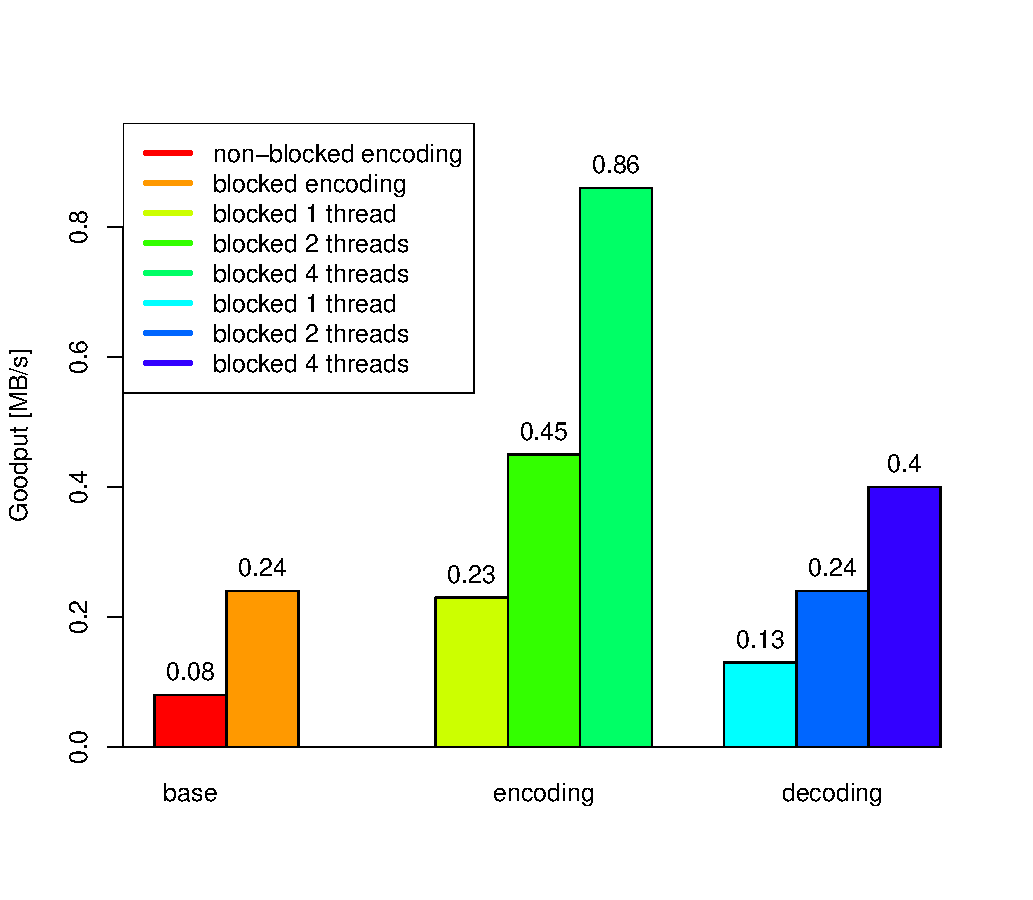
\includegraphics[width=0.7\textwidth]{images/2015-04-18_encoding_decoding_1024.pdf}
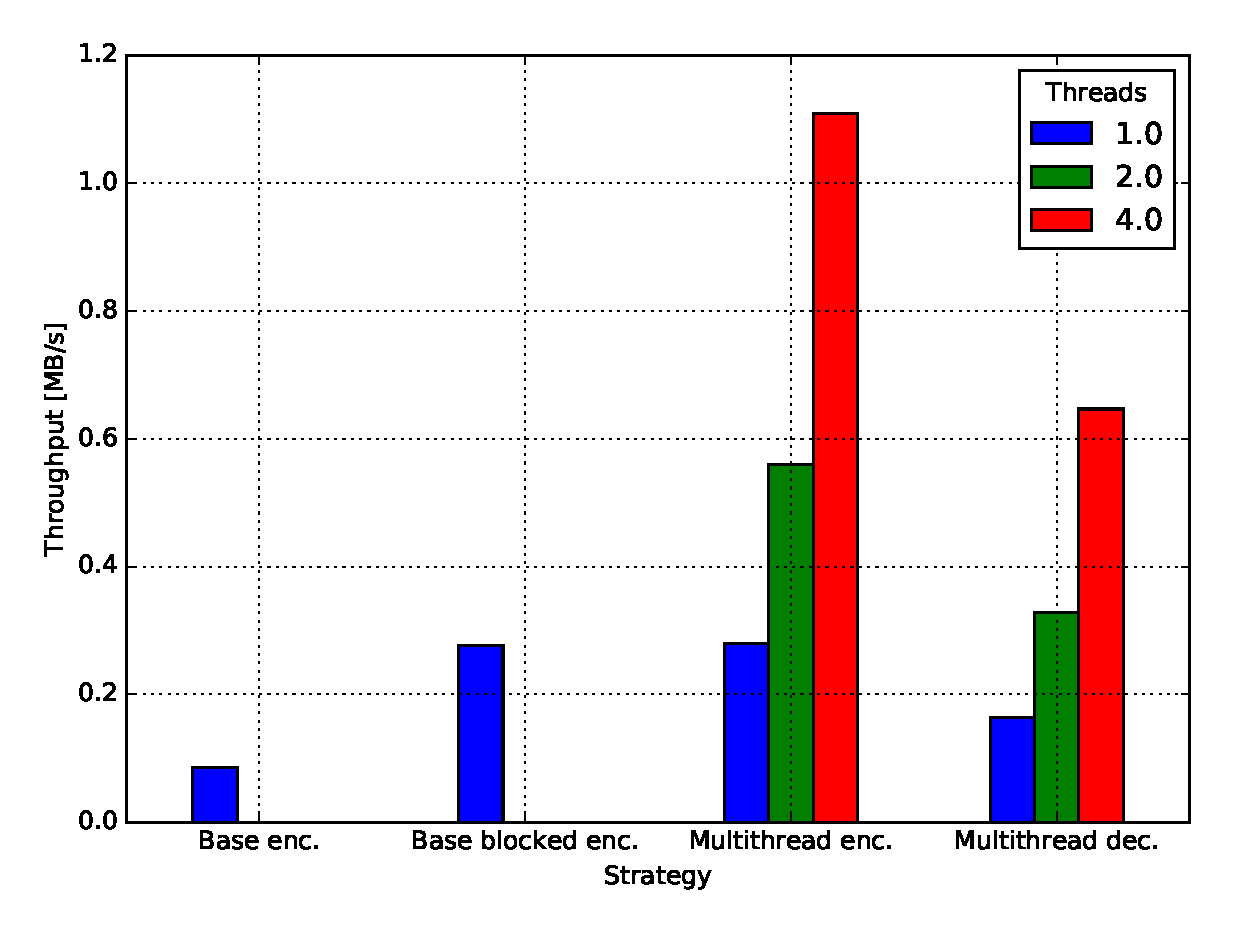
\includegraphics[width=0.7\textwidth]{images/GenSize_1024_SymbolSize_1536.eps}
\caption{Encoding and Decoding performance for $g = 1024$. Block size: $128 \times 128$.}
\label{enc_dec1024}
\end{figure}

For $g= 1024$, the blocked baseline measurements outperforms the non blocked
variant. This means that making the matrix multiplication algorithm cache
efficient brings an increase in goodput by a factor of 3.24. When using the
algorithm described in Section~\ref{sub:implementation-multicore}, encoding with
four cores is on average $3.9\times$ faster than with one core. Similarly,
decoding with four codes is $3.9\times$ faster, on average, than decoding with
a single core. Fig.~\ref{enc_dec1024} shows that the implemented algorithm, by
exploiting cache efficiency and only three extra cores provides a $13\times$
gain compared with traditional non-blocked algorithms. With $g = 1024$, the
matrix inversion becomes more expensive than at smaller generations sizes.
Therefore, the decoding goodput is 58\% of the encoding goodput.

\begin{figure}[ht!]
\centering
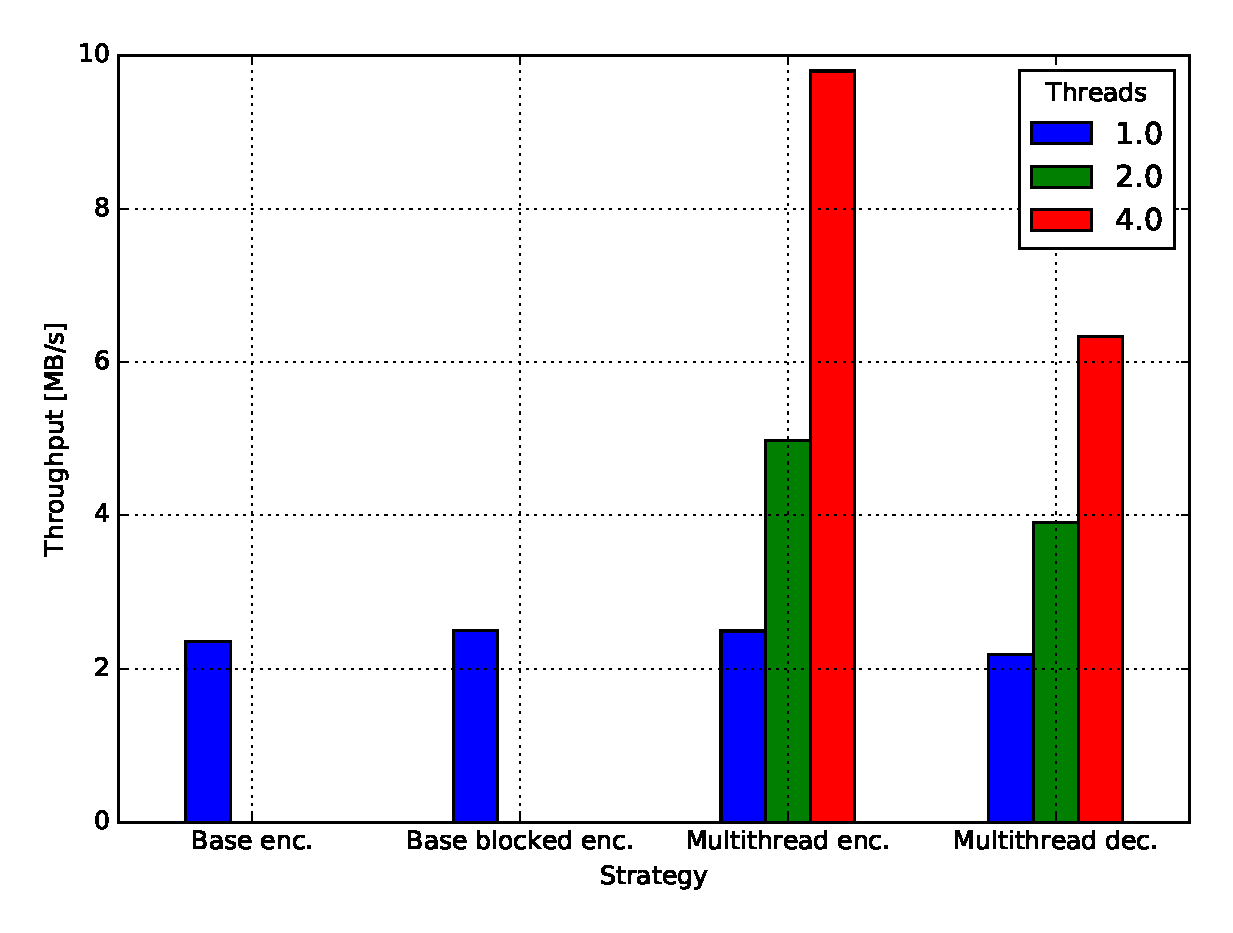
\includegraphics[width=0.7\textwidth]{images/GenSize_128_SymbolSize_1536.eps}
\caption{Encoding and Decoding performance for $g = 128$. Block size: $128 \times 128$}
\label{enc_dec128}
\end{figure}

For $g = 128$, the differences between the baselines operations show that a
blocked algorithm is 8\% faster than the non-blocked variant. Encoding with
four cores is $2.89\times$ faster than with a single core. Due to the smaller
matrix sizes, the gain when using blocked operations in the baselines is not
that significant when compared with $g = 1024$. For the same reason, the matrix
inversion is less expensive. As a consequence, the decoding goodput is 46\%
of the encoding goodput.

\begin{figure}[ht!]
\centering
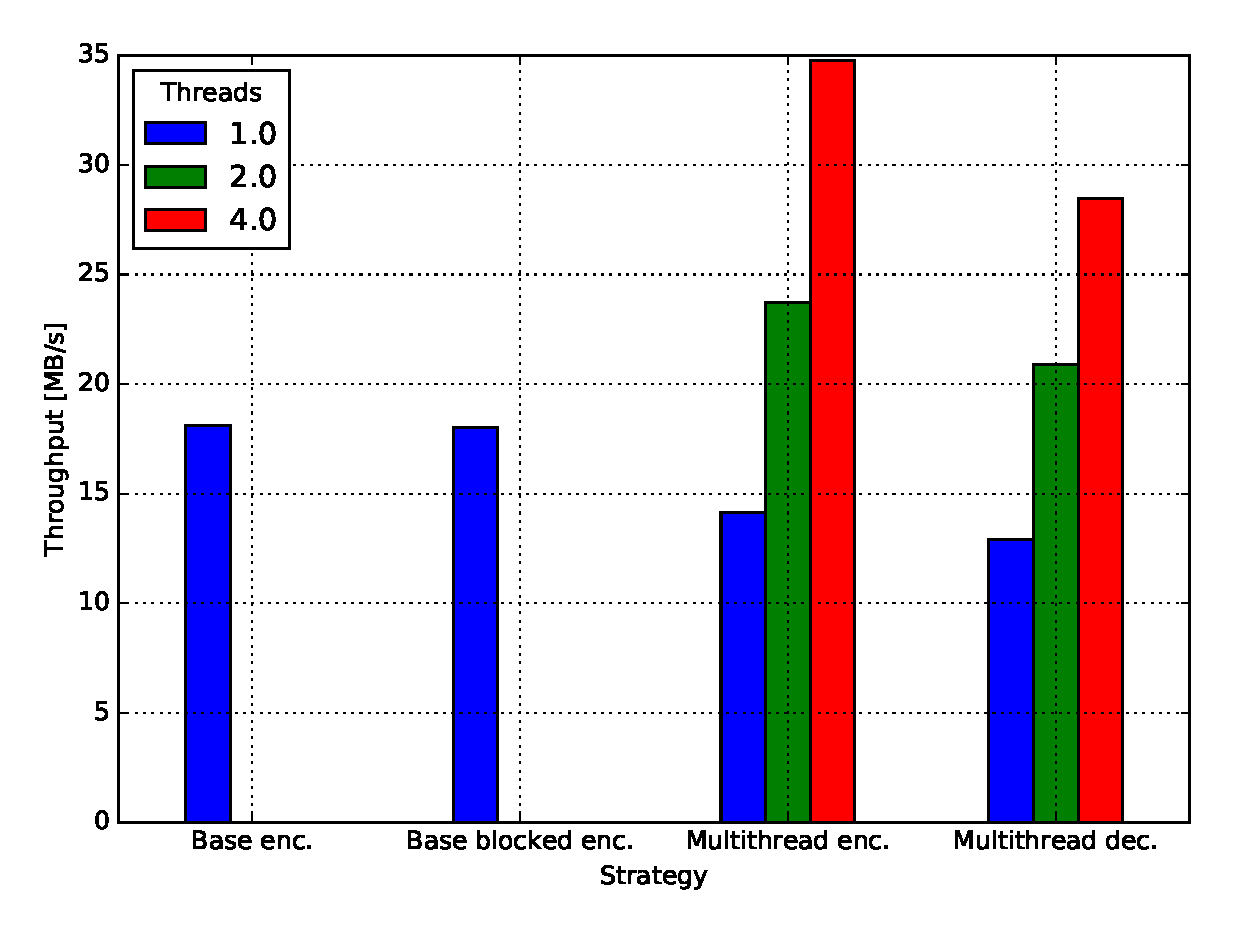
\includegraphics[width=0.7\textwidth]{images/GenSize_16_SymbolSize_1536.eps}
\caption{Encoding and Decoding performance for $g = 16$. Block size: $16 \times 16$}
\label{enc_dec16}
\end{figure}

When $g = 16$, the gains of blocked operations are negligible compared with
the non-blocked ones. The reason behind this behavior is that all the data
fits in the L1 cache. For the scheduled version, since the problem to solve
is so small, the gain when using four cores is a factor of 2.45 compared
with a single core, and 1.46 compared with two cores. Therefore, the
practical benefits in using four cores instead of two are reduced.

The differences in goodput, for all generation sizes, between the
blocked baseline and the single threaded scheduled measurements are due the
time spent resolving the dependencies and the scheduling overhead. These
effects are negligible for big generation sizes, while considerable for
small matrices. For instance, Fig.~\ref{enc_dec16} shows that the encoding
speed when using one core with the described algorithm is 78\% the encoding
speed without the recording and calculation of the \ac{DAG}.

\subsubsection{Comparison of the load of matrix multiplications and inversions}

To compare how much slower is the matrix multiplication with respect to the
matrix inversion for different generation sizes, we ran a set of tests. We used
a single core to perform the operations. We changed the generation sizes,
performed matrices multiplications and matrix inversions, and measured the time
spent doing so which we name $T_{mult}$ and $T_{inv}$. We calculate the ratio
between these two measured times defined as $r = \frac{T_{mult}}{T_{inv}}$.
Table~\ref{runtimes} summarizes the results. The bigger the matrix size, the
smaller is the calculated ratio. This means that when the problems are bigger,
the decoding goodput decreases compared with the encoding goodput.

\begin{table}[H]
\center
\caption{Multiplication and inversion run-times for different generation sizes with 1 thread}
\begin{tabular}{|r|r|r|r|}

\hline
$g$ & $T_{mult}$ (ms) & $T_{inv}$ (ms) &$r$ \\
\hline
\hline

	16   & 1.495     & 0.169    & 8.8 \\
\hline
	32   & 5.365     & 0.514    & 10.4 \\
\hline
	64   & 20.573    & 2.024    & 10.1 \\
\hline
	128  & 81.357    & 11.755   & 6.9 \\
\hline
	256  & 326.587   & 75.451  & 4.3 \\
\hline
	512  & 1354.012  & 540.469  & 2.5 \\
\hline
	1024 & 5965.284  & 4373.329 & 1.3 \\
\hline
\end{tabular}
\vspace{0.2cm}
\label{runtimes}
\end{table}


\section{Conclusion}
\label{sec:conclusions}
Given the usefulness of the \ac{Raspi} as a low-complex
processing node in large-scale networks and network coding
techniques against state-of-the-art routing, we provide
a performance evaluation of network coding schemes focusing on
processing speed and energy consumption for two \ac{Raspi} models.
The evaluation includes algorithms that exploit both \ac{SIMD}
instructions and multicore capabilities of the \ac{Raspi} 2. Our
measurements show that processing speeds of more than 80 Mbps and 800
Mbps are attainable for the \ac{Raspi} model 1 and 2, respectively,
for a wide range of network coding configurations and maintaining
a processing energy below 1 nJ/bit (or even an order of magnitude lower)
in similar configurations. For the use of multithreading, we quantify
processing gains ranging from 2$\times$ for $g = 16$ to 13$\times$ for
$g = 1024$ when employing 4 threads each in a different core. Future
work in the use of \ac{Raspi} devices will focus on considering: (i)
the performance of the \ac{Raspi} in scenarios with synthetic packet
losses, (ii) wireless networks where real packet losses can occur
and (iii) other topologies such as broadcast or
cooperative scenario to compare with theoretical results in order to
evaluate the performance of different network codes with the \ac{Raspi}.


%%%%%%%%%%%%%%%%%%%%%%%%%%%%%%%%%%%%%%%%%%
% \subsection{Subsection}
% \subsubsection{Subsubsection}

% Bulleted lists look like this:
% \begin{itemize}[leftmargin=*,labelsep=4mm]
% \item	First bullet
% \item	Second bullet
% \item	Third bullet
% \end{itemize}

% Numbered lists can be added as follows:
% \begin{enumerate}[leftmargin=*,labelsep=3mm]
% \item	First item
% \item	Second item
% \item	Third item
% \end{enumerate}

% The text continues here.

% \subsection{Figures, Tables and Schemes}

% All figures and tables should be cited in the main text as Figure 1, Table 1, etc.

% \begin{figure}[H]
% \centering
% %\includegraphics[width=3cm]{logo-mdpi}
% \caption{This is a figure, Schemes follow the same formatting. If there are multiple panels, they should be listed as: (\textbf{a}) Description of what is contained in the first panel. (\textbf{b}) Description of what is contained in the second panel. Figures should be placed in the main text near to the first time they are cited. A caption on a single line should be centered.}
% \end{figure}

% \begin{table}[H]
% \caption{This is a table caption. Tables should be placed in the main text near to the first time they are cited.}
% \small % Font size can be changed to match table content. Recommend 10 pt.
% \centering
% \begin{tabular}{ccc}
% \toprule
% \textbf{Title 1}	& \textbf{Title 2}	& \textbf{Title 3}\\
% \midrule
% entry 1		& data			& data\\
% entry 2		& data			& data\\
% \bottomrule
% \end{tabular}
% \end{table}

% \subsection{Formatting of Mathematical Components}

% This is an example of an equation:

% \begin{equation}
% \mathbb{S}
% \end{equation}

%% If the documentclass option "submit" is chosen, please insert a blank line before and after any math environment (equation and eqnarray environments). This ensures correct linenumbering. The blank line should be removed when the documentclass option is changed to "accept" because the text following an equation should not be a new paragraph.
% Please punctuate equations as regular text. Theorem-type environments (including propositions, lemmas, corollaries etc.) can be formatted as follows:
%% Example of a theorem:
% \begin{Theorem}
% Example text of a theorem.
% \end{Theorem}
% The text continues here. Proofs must be formatted as follows:

%% Example of a proof:
% \begin{proof}[Proof of Theorem 1]
% Text of the proof. Note that the phrase `of Theorem 1' is optional if it is clear which theorem is being referred to.
% \end{proof}
% The text continues here.

%%%%%%%%%%%%%%%%%%%%%%%%%%%%%%%%%%%%%%%%%%
%\section{Discussion}

%This section may be divided by subheadings. Authors should discuss the results and how they can be interpreted in perspective of previous studies and of the working hypotheses. The findings and their implications should be discussed in the broadest context possible. Future research directions may also be highlighted.

%%%%%%%%%%%%%%%%%%%%%%%%%%%%%%%%%%%%%%%%%%
%\section{Materials and Methods}

%This section should be divided by subheadings. Materials and Methods should be described with sufficient details to allow others to replicate and build on published results. Please note that publication of your manuscript implicates that you must make all materials, data, and protocols associated with the publication available to readers. Please disclose at the submission stage any restrictions on the availability of materials or information. New methods and protocols should be described in detail while well-established methods can be briefly described and appropriately cited.

%Research manuscripts reporting large datasets that are deposited in a publicly available database should specify where the data have been deposited and provide the relevant accession numbers. If the accession numbers have not yet been obtained at the time of submission, please state that they will be provided during review. They must be provided prior to publication.

%%%%%%%%%%%%%%%%%%%%%%%%%%%%%%%%%%%%%%%%%%
%\section{Conclusions}

%This section is not mandatory, but can be added to the manuscript if the discussion is unusually long or complex.

%%%%%%%%%%%%%%%%%%%%%%%%%%%%%%%%%%%%%%%%%%
\vspace{6pt}

%%%%%%%%%%%%%%%%%%%%%%%%%%%%%%%%%%%%%%%%%%
%% optional
% \supplementary{The following are available online at www.mdpi.com/link, Figure S1: title, Table S1: title, Video S1: title.}

%%%%%%%%%%%%%%%%%%%%%%%%%%%%%%%%%%%%%%%%%%
\acknowledgments{This research has been partially financed by the
Marie Curie Initial Training Network (ITN) CROSSFIRE project
(Grant No. EU - FP7 - CROSSFIRE - 317126) from the European Comission FP7
framework, the Green Mobile Cloud project (Grant No. DFF - 0602 - 01372B),
the TuneSCode project (Grant No. DFF - 1335 - 00125) both granted by the
Danish Council for Independent Research (Det Frie Forskningsr\r{a}d), and
by the German Research Foundation (DFG) within the Collaborative Research
Center SFB 912 – HAEC.}

%All sources of funding of the study should be disclosed. Please clearly indicate grants that you have received in support of your research work. Clearly state if you received funds for covering the costs to publish in open access.

%%%%%%%%%%%%%%%%%%%%%%%%%%%%%%%%%%%%%%%%%%
% \authorcontributions{For research articles with several authors, a short paragraph specifying their individual contributions must be provided. The following statements should be used ``X.X. and Y.Y. conceived and designed the experiments; X.X. performed the experiments; X.X. and Y.Y. analyzed the data; W.W. contributed reagents/materials/analysis tools; Y.Y. wrote the paper.'' Authorship must be limited to those who have contributed substantially to the work reported.}

%%%%%%%%%%%%%%%%%%%%%%%%%%%%%%%%%%%%%%%%%%
\conflictofinterests{The authors declare no conflict of interest. The founding sponsors had no role in the design of the study; in the collection, analyses, or interpretation of data; in the writing of the manuscript, and in the decision to publish the results.}

%Declare conflicts of interest or state ``The authors declare no conflict of interest.'' Authors must identify and declare any personal circumstances or interest that may be perceived as inappropriately influencing the representation or interpretation of reported research results. Any role of the funding sponsors in the design of the study; in the collection, analyses or interpretation of data; in the writing of the manuscript, or in the decision to publish the results must be declared in this section. If there is no role, please state ``The founding sponsors had no role in the design of the study; in the collection, analyses, or interpretation of data; in the writing of the manuscript, and in the decision to publish the results''.

%%%%%%%%%%%%%%%%%%%%%%%%%%%%%%%%%%%%%%%%%%
%% optional

% Use these two commands to get used acronyms
%used=$(grep -ohR '\\ac{[^}]*' *.tex | cut -f2 -d'{' | sort | uniq)
%for ac in ${used[@]}; do echo "$(grep -R "acro{${ac}}" acronym.tex)"; done | cut -f2-4 -d'{'
% Use text editor to replace '}{' --> ': ' and '}' --> '\\'

\abbreviations{The following abbreviations are used in this manuscript:\\

\noindent
ARM: Advanced RISC Machine\\
BLAS: Basic Linear Algebra Subprograms\\
CPU: Central Processing Unit\\
D2D: Device to Device\\
DAG: Direct Acyclic Graph\\
DC: Direct Current\\
dof: degrees of freedom\\
GB: Gigabyte\\
GF: Galois Field\\
GPU: Graphic Processing Unit\\
IoT: Internet of Things\\
IP: Internet Protocol\\
IP: Internet Protocol\\
LAN: Local Area Network\\
%l.d.: linearly dependent\\
LDPC: Low Density Parity Check\\
%l.i.: linearly independent\\
MAC: Medium Access Control\\
NC: Network Coding\\
NFS: Network File System\\
OS: Operating System\\
PC: Personal Computer\\
QoE: Quality of Experience\\
RAM: Random Access Memory\\
Raspi: Raspberry Pi\\
RLNC: Random Linear Network Coding\\
SCP: Secure copy\\
SIMD: Single Instruction Multiple Data\\
SIMD: Single Instruction Multiple Data\\
SMP: Symmetric Multiprocessor\\
SOC: System on Chip\\
SRLNC: Sparse Random Linear Network Coding\\
SSH: Secure Shell\\
Telnet: Telnet\\
TSNC: Tunable Sparse Network Coding\\
USB: Universal Serial Bus}

%%%%%%%%%%%%%%%%%%%%%%%%%%%%%%%%%%%%%%%%%%
%% optional
% \appendix
% \section{}
% The appendix is an optional section that can contain details and data supplemental to the main text. For example, explanations of experimental details that would disrupt the flow of the main text, but nonetheless remain crucial to understanding and reproducing the research shown; figures of replicates for experiments of which representative data is shown in the main text can be added here if brief, or as Supplementary data. Mathemtaical proofs of results not central to the paper can be added as an appendix.

% \section{}
% All appendix sections must be cited in the main text. In the appendixes, Figures, Tables, etc. should be labeled starting with `A', e.g., Figure A1, Figure A2, etc.

%%%%%%%%%%%%%%%%%%%%%%%%%%%%%%%%%%%%%%%%%%
\bibliographystyle{mdpi}

%=====================================
% References, variant A: internal bibliography
%=====================================
% \renewcommand\bibname{References}
% \begin{thebibliography}{999}
% % Reference 1
% \bibitem{ref-journal}
% Lastname, F.; Author, T. The title of the cited article. {\em Journal Abbreviation} {\bf 2008}, {\em 10}, 142-149.
% % Reference 2
% \bibitem{ref-book}
% Lastname, F.F.; Author, T. The title of the cited contribution. In {\em The Book Title}; Editor, F., Meditor, A., Eds.; Publishing House: City, Country, 2007; pp. 32-58.
% \end{thebibliography}

%=====================================
% References, variant B: external bibliography
%=====================================
\bibliography{raspi_journal}

%%%%%%%%%%%%%%%%%%%%%%%%%%%%%%%%%%%%%%%%%%
%% optional
\sampleavailability{The testbed and measurements in this publication are both available from the authors.}

%%%%%%%%%%%%%%%%%%%%%%%%%%%%%%%%%%%%%%%%%%
\end{document}
